\documentclass[12pt,a4paper]{article}
\usepackage[utf8]{inputenc}
\usepackage[english]{babel}
\usepackage{amsmath}
\usepackage{amsfonts}
\usepackage{amssymb}
\usepackage{graphicx}
\usepackage{float}
\usepackage{hyperref}
\usepackage{booktabs}
\usepackage{array}
\usepackage{multirow}
\usepackage{geometry}
\usepackage{fancyhdr}
\usepackage{subcaption}

% Page setup
\geometry{left=2.5cm,right=2.5cm,top=2.5cm,bottom=2.5cm}
\pagestyle{fancy}
\fancyhf{}
\rhead{\thepage}
\lhead{CNN for Rock-Paper-Scissors Classification}

% Hyperref setup
\hypersetup{
    colorlinks=true,
    linkcolor=black,
    filecolor=black,      
    urlcolor=blue,
    citecolor=black,
    pdftitle={Rock-Paper-Scissors CNN Classification Report},
}

\begin{document}

% Title page
\begin{titlepage}
\centering
\vspace*{2cm}

{\huge\textbf{Convolutional Neural Networks for}\par}
\vspace{0.5cm}
{\huge\textbf{Rock-Paper-Scissors Classification}\par}
\vspace{1cm}


\vspace{2cm}
\rule{\textwidth}{0.5pt}
\vspace{0.5cm}

{\large
\begin{tabular}{rl}
\textbf{Student:} & Dias Kalyshev \\[0.2cm]
\textbf{Student ID:} & 60641A \\[0.2cm]
\textbf{Course:} & Machine Learning  \\[0.2cm]
\textbf{Professor:} & Cesa Bianchi \\[0.2cm]
\textbf{Date:} & February 2026 \\
\end{tabular}
}

\vspace{0.5cm}
\rule{\textwidth}{0.5pt}

\vfill

\begin{minipage}{0.9\textwidth}
\setlength{\parindent}{0pt}
\setlength{\parskip}{0.5em}

\textbf{Abstract:} This report presents a comprehensive comparative study of main three convolutional neural network (CNN) architectures for rock-paper-scissors hand gesture classification, with emphasis on different evaluation methodologies. Three models were implemented with incremental complexity: SimplestCNN (2 convolutional layers), MediumCNN (4 layers), and DeepCNN (6 layers). All models were trained on the Kaggle Rock-Paper-Scissors dataset (2,188 images) using systematic data augmentation and hyperparameter optimization through grid search across 27 configurations.

The study employed rigorous methodology including stratified train/validation/test splits (70\%/10\%/20\%), comprehensive data augmentation, and extensive evaluation using multiple metrics: accuracy, precision, recall, F1-score, confusion matrices, ROC curves with AUC analysis, and detailed misclassification pattern visualization. Hyperparameter optimization identified optimal settings: learning rate 0.001, batch size 64, dropout 0.5, achieving 97.72\% validation accuracy.

Results reveal that SimplestCNN with hyperparameter tuning achieved the highest test accuracy (96.35\%) in 433s training time, outperforming MediumCNN (93.38\%, 581s) and DeepCNN (95.66\%, 1,038s). DeepCNN demonstrated exceptional discriminative ability with near-perfect ROC-AUC scores (0.995-1.000 across all classes). However, evaluation on 21 custom real-world images exposed severe generalization challenges, with DeepCNN accuracy dropping to 38.10\% (57.56 percentage point gap). Per-class analysis revealed particularly poor rock gesture recognition (14.29\% custom accuracy against 96.58\% test accuracy).

This study validates sound machine learning methodology while revealing the substantial gap between controlled test performance and real-world applicability.

\end{minipage}

\vspace{1cm}

\end{titlepage}

% Declaration page
\newpage
\thispagestyle{empty}
\vspace*{2cm}

\section*{Declaration}

I declare that this material, which I now submit for assessment, is entirely my own work and has not been taken from the work of others, save and to the extent that such work has been cited and acknowledged within the text of my work. I understand that plagiarism, collusion, and copying are grave and serious offences in the university and accept the penalties that would be imposed should I engage in plagiarism, collusion or copying. This assignment, or any part of it, has not been previously submitted by me or any other person for assessment on this or any other course of study.


\newpage

\tableofcontents
\newpage

\section{Introduction}

\subsection{Problem Statement and Motivation}

Hand gesture recognition represents a fundamental challenge in computer vision with applications spanning gaming interfaces, human-computer interaction, robotics, sign language interpretation, and touchless control systems. This project focuses on classifying three hand gestures corresponding to the rock-paper-scissors game, which serves as an ideal benchmark problem for gesture recognition research.

The rock-paper-scissors classification task provides a well-defined structure with three distinct, mutually exclusive classes that possess clear semantic differences. This problem has direct practical applications in gaming interfaces, gesture-based controls, and interactive entertainment systems. Despite the apparent simplicity of three-class classification, the task presents significant real-world challenges including:

\begin{itemize}
    \item \textbf{Intra-class variability:} Hand size, shape, orientation, and positioning vary within each gesture class across different individuals and even multiple performances by the same person.
    \item \textbf{Inter-individual differences:} People execute gestures with naturally different styles, finger configurations, and hand proportions.
    \item \textbf{Environmental variations:} Background complexity, lighting conditions, shadows, and occlusions introduce substantial variability not present in controlled datasets.
    \item \textbf{Camera factors:} Perspective, viewing angle, distance, resolution, and focal length variations alter the appearance of gestures.
    \item \textbf{Temporal consistency:} Systems must maintain stable predictions across subtle hand position changes rather than flickering between classes.
\end{itemize}

Furthermore, this problem offers substantial educational value as an accessible entry point for understanding CNN architecture design, evaluation methodologies, and the critical gap between test set performance and real-world deployment readiness-a lesson that extends far beyond gesture recognition to virtually all applied machine learning.

\subsection{Research Objectives}

This study pursues six comprehensive objectives that extend beyond traditional accuracy-focused evaluations:

\textbf{1. Architectural Comparison:} Systematically compare three CNN architectures with 2, 4, and 6 convolutional layers to understand the relationship between model depth, complexity, and classification performance. Specifically investigate whether deeper networks provide advantages for this three-class problem or whether simpler architectures achieve comparable or superior results.

\textbf{2. Hyperparameter Optimization:} Conduct systematic hyperparameter optimization through grid search across 27 configurations, exploring combinations of learning rate (0.0001, 0.001, 0.01), batch size (32, 64, 128), and dropout rate (0.3, 0.5, 0.7) to identify optimal training settings. Document the sensitivity of model performance to these hyperparameters and establish best practices.

\textbf{3. Comprehensive Performance Evaluation:} Perform extensive evaluation using multiple metrics on standard test data including accuracy, precision, recall, F1-score, confusion matrices, ROC curves with AUC analysis, and detailed misclassification pattern identification. Move beyond single aggregate metrics to understand model behavior across different classes and error types.

\textbf{4. ROC Curve Analysis:} Investigate the discriminative power of each model through Receiver Operating Characteristic (ROC) curves and Area Under the Curve (AUC) metrics. Assess whether perfect or near-perfect AUC scores on test data translate to robust real-world performance, or whether they represent a misleading indicator of deployment readiness.

\textbf{5. Misclassification Pattern Analysis:} Conduct detailed investigation of error patterns through visualization of misclassified samples and systematic analysis of confusion pairs. Identify which gesture types are most frequently confused, understand the visual characteristics that lead to errors, and determine whether mistakes occur on genuinely ambiguous cases or clear instances that should be correctly classified.

\textbf{6. Real-World Generalization Assessment:} Evaluate generalization capability through testing on custom images captured under different conditions than the training data. Quantify the performance gap between in-distribution test data and out-of-distribution real-world images to assess true deployment readiness. Analyze class-specific vulnerabilities and identify which gesture types are most sensitive to distribution shift.

Through these objectives, the study demonstrates sound machine learning methodology including proper data splitting, augmentation strategies, rigorous multi-metric evaluation, and honest assessment of limitations-practices essential for developing deployable systems rather than merely models that perform well on standard benchmarks.

\subsection{Dataset Description}

\subsubsection{Primary Dataset}

The Rock-Paper-Scissors dataset from Kaggle contains 2,188 RGB images distributed nearly equally across three classes. The dataset composition demonstrates balanced class representation:

\begin{table}[H]
\centering
\begin{tabular}{lcc}
\toprule
\textbf{Class} & \textbf{Images} & \textbf{Percentage} \\
\midrule
Paper & 712 & 32.5\% \\
Rock & 726 & 33.2\% \\
Scissors & 750 & 34.3\% \\
\midrule
\textbf{Total} & \textbf{2,188} & \textbf{100\%} \\
\bottomrule
\end{tabular}
\caption{Class distribution in the primary dataset}
\end{table}

Images are stored in JPEG compressed format with variable dimensions, typically around 300×200 pixels. The dataset is characterized by:

\begin{itemize}
    \item Uniform white or light-colored backgrounds providing minimal visual complexity
    \item Centered hand gestures with consistent framing across images
    \item Controlled indoor lighting conditions that minimize shadows and artifacts
    \item Predominantly frontal viewing angles with hands positioned perpendicular to camera
    \item Limited variation in hand size, skin tone, and individual gesture execution styles
\end{itemize}

These characteristics create a relatively homogeneous distribution ideal for initial model training and validation but potentially limiting for generalization to diverse real-world conditions.

\begin{figure}[H]
    \centering
    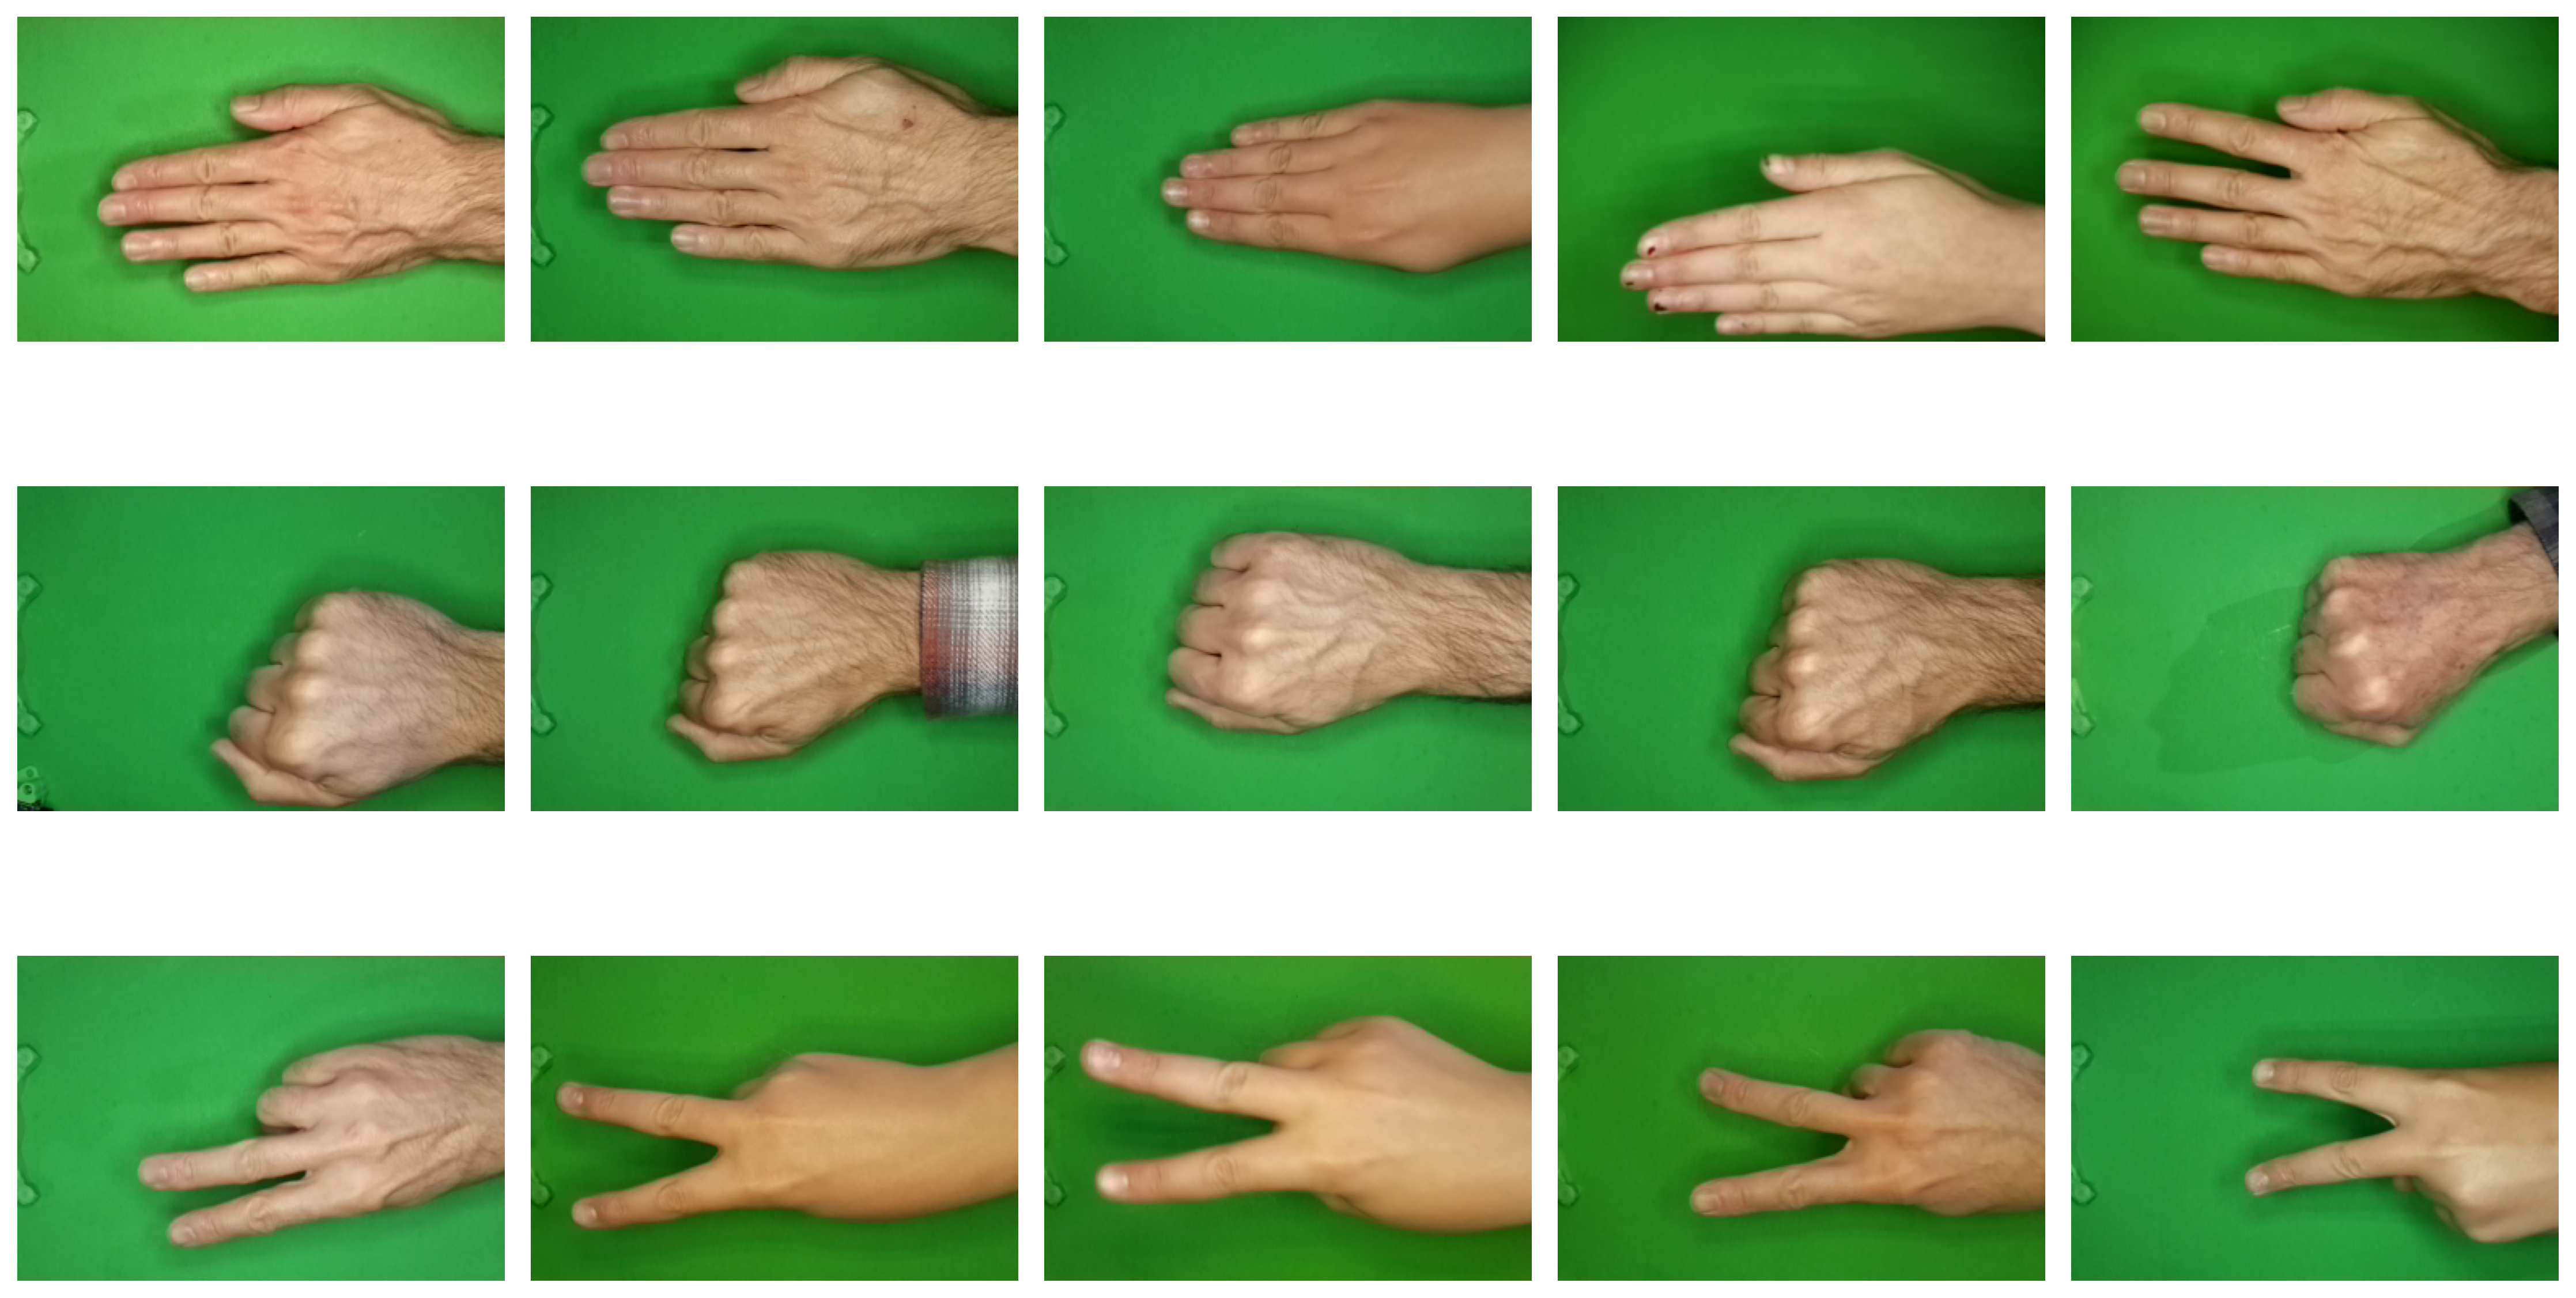
\includegraphics[width=0.95\textwidth]{figures/sample_images.png}
    \caption{Representative samples from each class showing typical hand gestures, framing, and background conditions in the training dataset. Note the consistent lighting, uniform backgrounds, and frontal viewing angles.}
    \label{fig:sample_images}
\end{figure}

\subsubsection{Data Splitting Strategy}

Stratified random splitting ensures balanced class representation across all subsets while maintaining statistical independence:

\begin{table}[H]
\centering
\begin{tabular}{lccp{6cm}}
\toprule
\textbf{Split} & \textbf{Percentage} & \textbf{Images} & \textbf{Purpose} \\
\midrule
Training & 70\% & 1,531 & Model optimization through gradient descent and weight updates \\
Validation & 10\% & 219 & Hyperparameter selection and early stopping decisions \\
Test & 20\% & 438 & Final unbiased evaluation of model performance \\
\midrule
\textbf{Total} & \textbf{100\%} & \textbf{2,188} & - \\
\bottomrule
\end{tabular}
\caption{Dataset split configuration with fixed random seed (42) for reproducibility}
\end{table}

The validation set remains strictly separate from training to provide unbiased hyperparameter evaluation and early stopping signals. The test set is used only once for final evaluation, preventing any form of indirect optimization on test data. All three splits maintain approximately equal class proportions through stratification.

\subsubsection{Custom Evaluation Dataset}

To assess real-world generalization capability beyond the standard test set, a custom evaluation dataset consisting of 21 images (7 per class) was created for testing. This custom dataset intentionally differs from the training distribution in several critical aspects:

\begin{itemize}
    \item \textbf{Background diversity:} Indoor scenes with various textures, colors, and variable lighting conditions rather than uniform backgrounds
    \item \textbf{Hand characteristics:} Different hand sizes, skin tones, and gesture execution styles across multiple individuals
    \item \textbf{Camera conditions:} Various angles, distances, and image quality characteristics to simulate realistic deployment scenarios
    \item \textbf{Lighting variation:} Natural lighting with shadows rather than controlled studio lighting
    \item \textbf{Positioning variability:} Hand positions not always perfectly centered, with varied orientations
\end{itemize}

This custom dataset serves as a crucial reality check for model robustness, revealing whether high test accuracy reflects genuine gesture recognition capability or merely memorization of training distribution characteristics. The substantial difference between training and custom conditions enables quantification of the generalization gap-a critical metric for assessing deployment readiness that standard test sets cannot provide.

\subsection{Contribution and Report Structure}

This report makes three primary contributions to understanding CNN-based gesture classification:

\textbf{1. Comprehensive Evaluation Methodology:} Demonstrates that standard accuracy metrics alone are insufficient for deployment assessment. Introduces multi-faceted evaluation combining ROC analysis, confusion matrices, misclassification visualization, and mandatory out-of-distribution testing.

\textbf{2. Architectural Simplicity Benefits:} Empirically demonstrates that the simplest architecture (2 convolutional layers, 84K parameters) outperforms deeper alternatives (4 and 6 layers, 215K and 850K parameters respectively) while requiring substantially less training time. Validates that appropriate problem-complexity matching often favors simpler models over architectural sophistication.

\textbf{3. Distribution Shift Vulnerability:} Documents that near-perfect test metrics (95.66\% accuracy, 0.995-1.000 ROC-AUC) completely fail to predict catastrophic real-world performance (38\% accuracy). Demonstrates that models learn distribution-specific patterns rather than robust gesture representations.

The remainder of this report is organized as follows:

\begin{itemize}
    \item \textbf{Section 2:} Detailed methodology covering data preprocessing, augmentation, architecture design, hyperparameter optimization, and evaluation metrics
    \item \textbf{Section 3:} Experimental results including training dynamics, test set performance with ROC analysis, and custom dataset evaluation
    \item \textbf{Section 4:} Discussion of model complexity trade-offs, generalization challenges, and evaluation methodology insights
    \item \textbf{Section 5:} Conclusions, practical recommendations, limitations, and future work directions
\end{itemize}

\section{Methodology}

\subsection{Data Preprocessing and Augmentation}

\subsubsection{Image Preprocessing Pipeline}

All images undergo standardized preprocessing to ensure consistent input formats for neural network processing:

\begin{enumerate}
    \item \textbf{Resizing:} Images are resized to 128×128 pixels to provide uniform dimensions across the dataset, balancing spatial resolution with computational efficiency
    \item \textbf{Normalization:} Pixel values are scaled to the [0, 1] range through division by 255, facilitating stable gradient computation during training
    \item \textbf{Tensor Conversion:} Images are converted to PyTorch tensor format with channels-first ordering (C×H×W), as required by PyTorch's convolutional layers
\end{enumerate}

This preprocessing pipeline ensures that the network receives consistently formatted inputs regardless of the original image dimensions or storage format.

\subsubsection{Data Augmentation Strategy}

Comprehensive data augmentation was applied exclusively to the training dataset to improve model generalization while maintaining the original distribution of validation and test sets for fair evaluation. The augmentation strategy encompasses two categories of transformations implemented using PyTorch's torchvision library.

\textbf{Geometric Transformations:}
\begin{itemize}
    \item \textbf{Random Rotation:} Images are randomly rotated within ±15 degrees to simulate varied hand orientations and viewing angles
    \item \textbf{Random Horizontal Flip:} Applied with 50\% probability to introduce left-right symmetry variations, though this transformation may not be semantically meaningful for gesture recognition where handedness matters
\end{itemize}

\textbf{Color Space Augmentations:}
\begin{itemize}
    \item \textbf{Color Jittering:} Brightness, contrast, saturation, and hue are adjusted by moderate factors (±0.2 for brightness/contrast/saturation, ±0.1 for hue) to simulate different lighting conditions and camera settings
    \item \textbf{Random Grayscale:} Applied with 10\% probability to improve robustness to color variations and encourage the model to rely on shape rather than color cues
\end{itemize}

All transformations are applied stochastically during training, with each image potentially receiving different augmentation parameters each time it is loaded. This approach effectively increases dataset diversity without requiring additional labeled data. Validation and test sets receive only resizing to 128×128 pixels and normalization without augmentation, preserving the original data distribution for unbiased performance assessment.

\subsection{Model Architectures}

Three CNN architectures with increasing complexity were implemented using PyTorch to investigate the relationship between model depth and performance.

\subsubsection{SimplestCNN (2 Convolutional Layers)}

The SimplestCNN architecture represents a lightweight design focusing on efficient feature extraction with minimal computational overhead. The network consists of two convolutional blocks followed by fully connected layers for classification.

\textbf{Architecture Specification:}

\textbf{Convolutional Block 1:}
\begin{itemize}
    \item Conv2D: 3->32 channels, 5×5 kernel, padding=2 (maintains spatial dimensions)
    \item BatchNorm2D(32): Normalizes activations for training stability
    \item ReLU activation: Introduces non-linearity
    \item MaxPool2D(2×2): Reduces spatial dimensions from 128×128 -> 64×64
\end{itemize}

\textbf{Convolutional Block 2:}
\begin{itemize}
    \item Conv2D: 32->64 channels, 5×5 kernel, padding=2
    \item BatchNorm2D(64): Further stabilizes learning
    \item ReLU activation
    \item MaxPool2D(2×2): Reduces dimensions from 64×64 -> 32×32
\end{itemize}

\textbf{Classification Head:}
\begin{itemize}
    \item AdaptiveAvgPool2D(4×4): Produces fixed 4×4 spatial output regardless of input variations
    \item Flatten: Converts 64×4×4 feature maps to 1024-dimensional vector
    \item Linear(1024->128) + ReLU + Dropout(0.3): First fully connected layer with regularization
    \item Linear(128->3): Final classification layer producing class logits
\end{itemize}

The complete architecture contains approximately \textbf{84,000 trainable parameters}, making it highly efficient for training and inference. Despite its simplicity, this model achieved the highest test accuracy (96.35\%) among all architectures.

\subsubsection{MediumCNN (4 Convolutional Layers)}

The MediumCNN architecture represents a balanced design with progressive feature extraction through four convolutional blocks. This architecture employs smaller 3×3 kernels compared to SimplestCNN, allowing for more localized feature detection.

\textbf{Architecture Specification:}

\textbf{Four Convolutional Blocks:}
\begin{itemize}
    \item Block 1: 3->32 channels (3×3 kernel, padding=1)
    \item Block 2: 32->64 channels (3×3 kernel, padding=1)
    \item Block 3: 64->128 channels (3×3 kernel, padding=1)
    \item Block 4: 128->128 channels (3×3 kernel, padding=1)
\end{itemize}

Each block follows the pattern: Conv2D -> BatchNorm2D -> ReLU -> MaxPool2D(2×2)

\textbf{Classification Head:}
\begin{itemize}
    \item AdaptiveAvgPool2D(2×2): Produces fixed 2×2 spatial output
    \item Flatten: Converts 128×2×2 feature maps to 512-dimensional vector
    \item Linear(512->256) + ReLU + Dropout(0.4)
    \item Linear(256->128) + ReLU + Dropout(0.4)
    \item Linear(128->3): Final classification layer
\end{itemize}

The architecture contains approximately \textbf{215,000 trainable parameters}, representing a middle ground between SimplestCNN and DeepCNN. However, this model achieved the lowest test accuracy (93.38\%) despite increased complexity.

\subsubsection{DeepCNN (6 Convolutional Layers)}

The DeepCNN architecture represents the most sophisticated model in this study, employing six convolutional layers organized into three blocks with double convolutions. This design draws inspiration from VGG networks, using repeated 3×3 convolutions within each block.

\textbf{Architecture Specification:}

\textbf{Three Double-Convolution Blocks:}
\begin{itemize}
    \item Block 1: Two Conv2D layers (3->32->32 channels, 3×3 kernels)
    \item Block 2: Two Conv2D layers (32->64->64 channels, 3×3 kernels)
    \item Block 3: Two Conv2D layers (64->128->128 channels, 3×3 kernels)
\end{itemize}

Each block applies: Conv2D -> BatchNorm2D -> ReLU -> Conv2D -> BatchNorm2D -> ReLU -> MaxPool2D(2×2)

The double convolution strategy allows the network to learn more complex feature combinations before reducing spatial dimensions through pooling.

\textbf{Classification Head:}
\begin{itemize}
    \item AdaptiveAvgPool2D(4×4): Produces fixed 4×4 spatial output, yielding 2048 features after flattening
    \item Linear(2048->512) + ReLU + Dropout(0.5)
    \item Linear(512->256) + ReLU + Dropout(0.5)
    \item Linear(256->3): Final classification layer
\end{itemize}

The complete architecture contains approximately \textbf{850,000 trainable parameters}, representing 10× the parameters of SimplestCNN. This model achieved 95.66\% test accuracy and near-perfect ROC-AUC scores (0.995-1.000), but failed catastrophically on real-world custom images (38.10\%).

\textbf{Common Design Elements:}

All three architectures share several design principles:
\begin{itemize}
    \item \textbf{Batch Normalization:} Applied after each convolutional layer to stabilize training and accelerate convergence
    \item \textbf{Dropout Regularization:} Prevents overfitting through random neuron deactivation, with rates varying by complexity (0.3 for SimplestCNN, 0.4 for MediumCNN, 0.5 for DeepCNN)
    \item \textbf{Adaptive Pooling:} Provides flexibility in handling different input dimensions by producing fixed-size outputs
    \item \textbf{ReLU Activation:} Introduces non-linearity while avoiding vanishing gradient problems
\end{itemize}

\subsection{Hyperparameter Optimization}

\subsubsection{Grid Search Methodology}

Comprehensive grid search was conducted across 27 hyperparameter configurations to identify optimal training settings. The search space explored three critical hyperparameters:

\begin{table}[H]
\centering
\begin{tabular}{lc}
\toprule
\textbf{Hyperparameter} & \textbf{Values Explored} \\
\midrule
Learning Rate & 0.0001, 0.001, 0.01 \\
Batch Size & 32, 64, 128 \\
Dropout Rate & 0.3, 0.5, 0.7 \\
\midrule
\textbf{Total Combinations} & \textbf{27} \\
\bottomrule
\end{tabular}
\caption{Hyperparameter search space for grid search optimization}
\end{table}

Each configuration was trained for 10 epochs on the SimplestCNN architecture using validation accuracy as the optimization objective. This systematic approach ensures comprehensive exploration of the hyperparameter space rather than relying on ad-hoc tuning.

\subsubsection{Optimization Results}

\begin{table}[H]
\centering
\begin{tabular}{cccc}
\toprule
\textbf{Learning Rate} & \textbf{Batch Size} & \textbf{Dropout} & \textbf{Val Accuracy} \\
\midrule
\textbf{0.001} & \textbf{64} & \textbf{0.5} & \textbf{97.72\%} \\
0.001 & 64 & 0.3 & 97.26\% \\
0.001 & 32 & 0.5 & 97.26\% \\
0.001 & 64 & 0.7 & 97.26\% \\
0.001 & 32 & 0.7 & 96.80\% \\
\bottomrule
\end{tabular}
\caption{Top 5 hyperparameter configurations ranked by validation accuracy. The optimal configuration achieved 97.72\% validation accuracy.}
\end{table}

\textbf{Key Findings from Hyperparameter Optimization:}

\begin{itemize}
    \item \textbf{Learning Rate 0.001 dominates:} All top configurations use learning rate 0.001, demonstrating robustness across other hyperparameter choices
    \item \textbf{Batch size impact:} Larger batch sizes (64, 128) generally outperformed smaller batches (32), likely due to more stable gradient estimates
    \item \textbf{Dropout sweet spot:} Rates between 0.3-0.5 provided optimal regularization, with extreme values showing degraded performance
    \item \textbf{Learning rate extremes fail:} Rate 0.01 caused training instability, while 0.0001 was overly conservative requiring prohibitively long training
\end{itemize}

\begin{figure}[H]
    \centering
    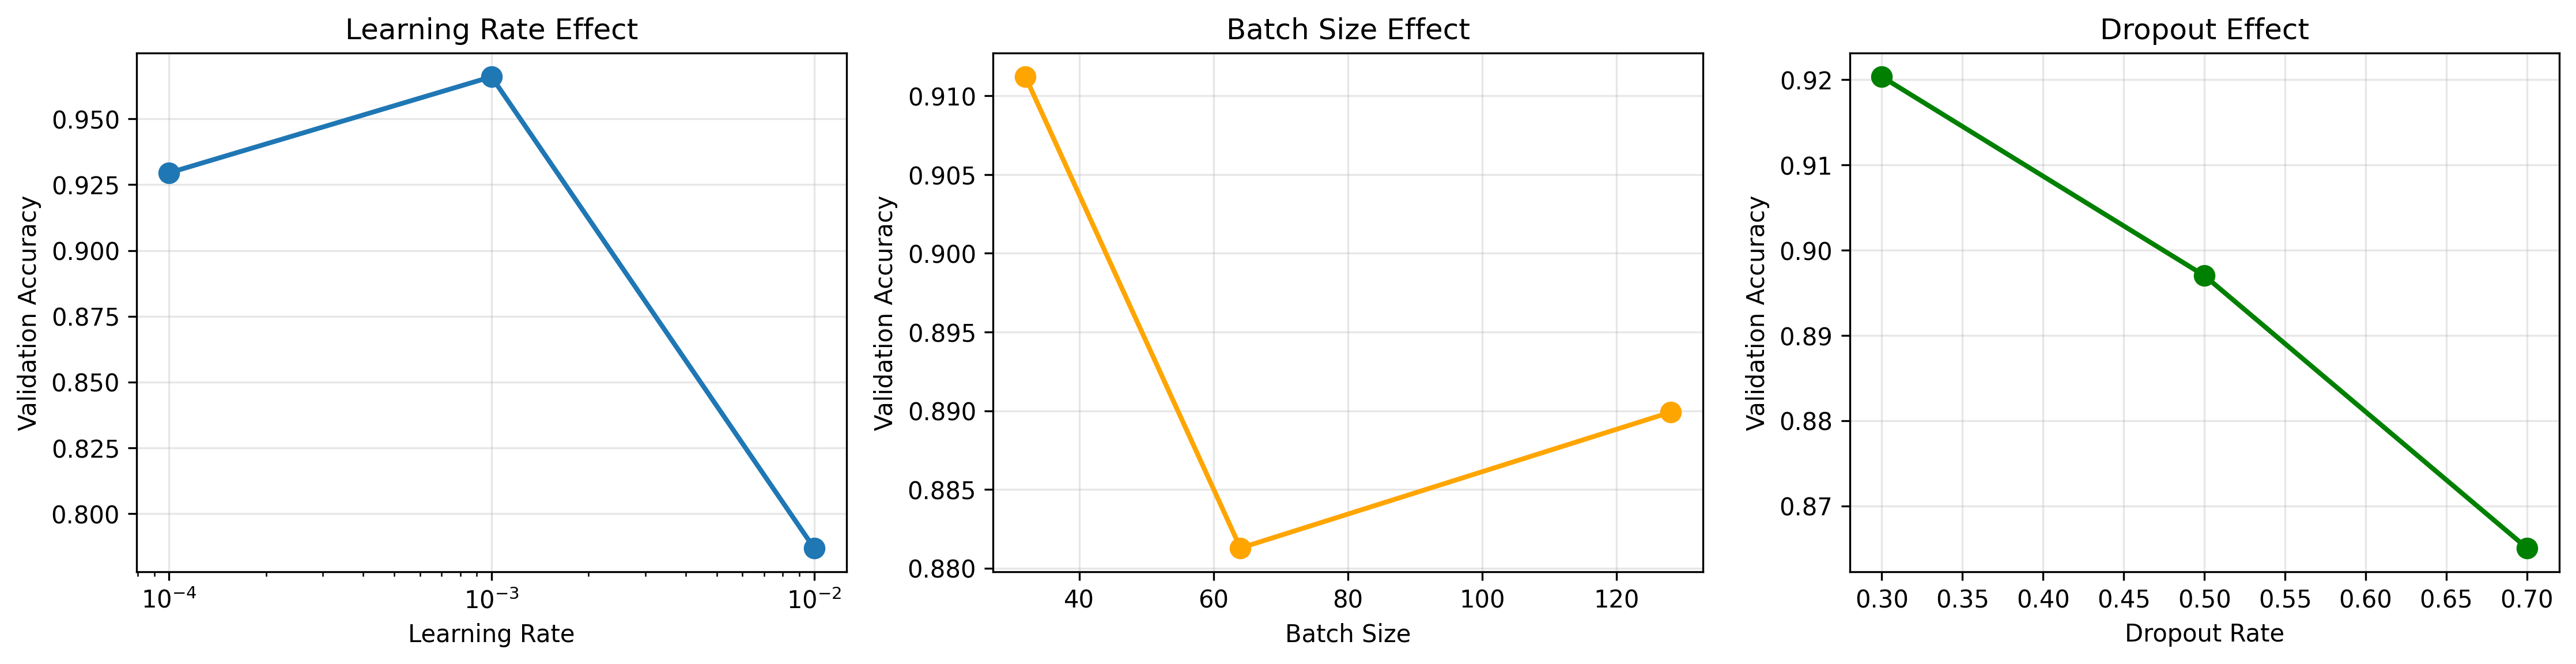
\includegraphics[width=0.85\textwidth]{figures/hyperparameter_effects.png}
    \caption{Validation accuracy across different hyperparameter combinations. Learning rate 0.001 consistently produces superior results across all batch size and dropout combinations.}
    \label{fig:hyperparameter_effects}
\end{figure}

The optimal configuration (learning rate 0.001, batch size 64, dropout 0.5) achieved 97.72\% validation accuracy, representing a \textbf{1.83 percentage point improvement} over baseline settings. This validates the investment in systematic hyperparameter search.

\subsection{Training Configuration}

\subsubsection{Training Parameters}

\begin{table}[H]
\centering
\begin{tabular}{ll}
\toprule
\textbf{Parameter} & \textbf{Value} \\
\midrule
Optimizer & Adam ($\beta_1$=0.9, $\beta_2$=0.999, $\varepsilon$=1$\times$10$^{-8}$) \\
Learning Rate & 0.001 (optimal from grid search) \\
Batch Size & 32 (SimplestCNN), 64 (Medium/DeepCNN) \\
Loss Function & CrossEntropyLoss \\
Max Epochs & 15 \\
Early Stopping & Patience of 5 epochs \\
Monitoring Metric & Validation Accuracy \\
Device & CPU \\
Random Seed & 42 (reproducibility) \\
\bottomrule
\end{tabular}
\caption{Final training configuration applied to all model architectures}
\end{table}

\subsubsection{Training Procedure}

The training procedure follows standard supervised learning protocol:

\begin{enumerate}
    \item \textbf{Initialization:} Model weights initialized randomly from normal distribution
    \item \textbf{Forward Pass:} Process batches of images through network layers to generate predictions
    \item \textbf{Loss Calculation:} CrossEntropyLoss compares predictions against ground truth labels
    \item \textbf{Backpropagation:} Compute gradients via automatic differentiation
    \item \textbf{Weight Update:} Adam optimizer updates parameters based on computed gradients
    \item \textbf{Validation:} After each epoch, evaluate on validation set without gradient updates
    \item \textbf{Early Stopping:} Monitor validation accuracy; halt if no improvement for 5 consecutive epochs
    \item \textbf{Model Saving:} Preserve model state achieving highest validation accuracy
\end{enumerate}

\subsection{Evaluation Metrics}

Comprehensive evaluation extends beyond single accuracy metrics to provide nuanced understanding of model behavior.

\subsubsection{Standard Classification Metrics}

\textbf{Accuracy:} Overall proportion of correct predictions across all classes

\textbf{Precision:} For each class, the proportion of predicted instances that are truly positive: $\text{Precision} = \frac{TP}{TP + FP}$

\textbf{Recall (Sensitivity):} For each class, the proportion of actual instances correctly identified: $\text{Recall} = \frac{TP}{TP + FN}$

\textbf{F1-Score:} Harmonic mean of precision and recall: $\text{F1} = 2 \times \frac{\text{Precision} \times \text{Recall}}{\text{Precision} + \text{Recall}}$

These metrics are computed both per-class and as weighted averages across all classes, accounting for class imbalance through support weighting.

\subsubsection{ROC Curves and AUC}

Receiver Operating Characteristic (ROC) curves visualize the trade-off between True Positive Rate (TPR) and False Positive Rate (FPR) across all possible classification thresholds. For multi-class problems, we compute:

\textbf{Per-Class ROC:} One-vs-rest approach treats each class independently against all others

\textbf{Micro-Average:} Aggregates contributions from all classes by computing TPR/FPR globally

\textbf{Macro-Average:} Computes ROC for each class independently, then averages

Area Under the Curve (AUC) quantifies discriminative ability, with values near 1.0 indicating perfect separation. However, as this study demonstrates, perfect AUC on test data does not guarantee real-world robustness when distribution shift occurs.

\subsubsection{Confusion Matrix Analysis}

Confusion matrices provide detailed class-level error patterns, revealing which gesture types are confused with which others. This enables targeted improvement strategies by identifying systematic failure modes.

\subsubsection{Misclassification Pattern Analysis}

Beyond aggregate metrics, we perform:
\begin{itemize}
    \item \textbf{Visual Inspection:} Display misclassified test images to understand failure characteristics
    \item \textbf{Confusion Pair Analysis:} Quantify specific error patterns (e.g., Scissors->Paper vs Scissors->Rock)
    \item \textbf{Per-Class Error Rates:} Identify which gestures are most vulnerable to misclassification
\end{itemize}

This detailed analysis reveals that on test data, 57.9\% of errors involve Scissors->Paper confusion, indicating inherent difficulty in distinguishing extended finger configurations.

\subsubsection{Out-of-Distribution Testing}

Standard test sets drawn from the training distribution cannot reveal robustness to distribution shift. Our custom dataset (21 real-world images) provides critical assessment of deployment readiness. This evaluation exposed severe generalization failure: \textbf{DeepCNN dropped from 95.66\% test accuracy to 38.10\% on custom images} (57.56 percentage point gap), with rock gestures catastrophically failing (14.29\% vs 96.58\%).

\section{Experimental Results}

\subsection{Training Dynamics}

\subsubsection{Baseline Training Convergence}

Figure \ref{fig:baseline_training} illustrates training and validation curves for the SimplestCNN architecture, demonstrating healthy convergence behavior without significant overfitting.

\begin{figure}[H]
    \centering
    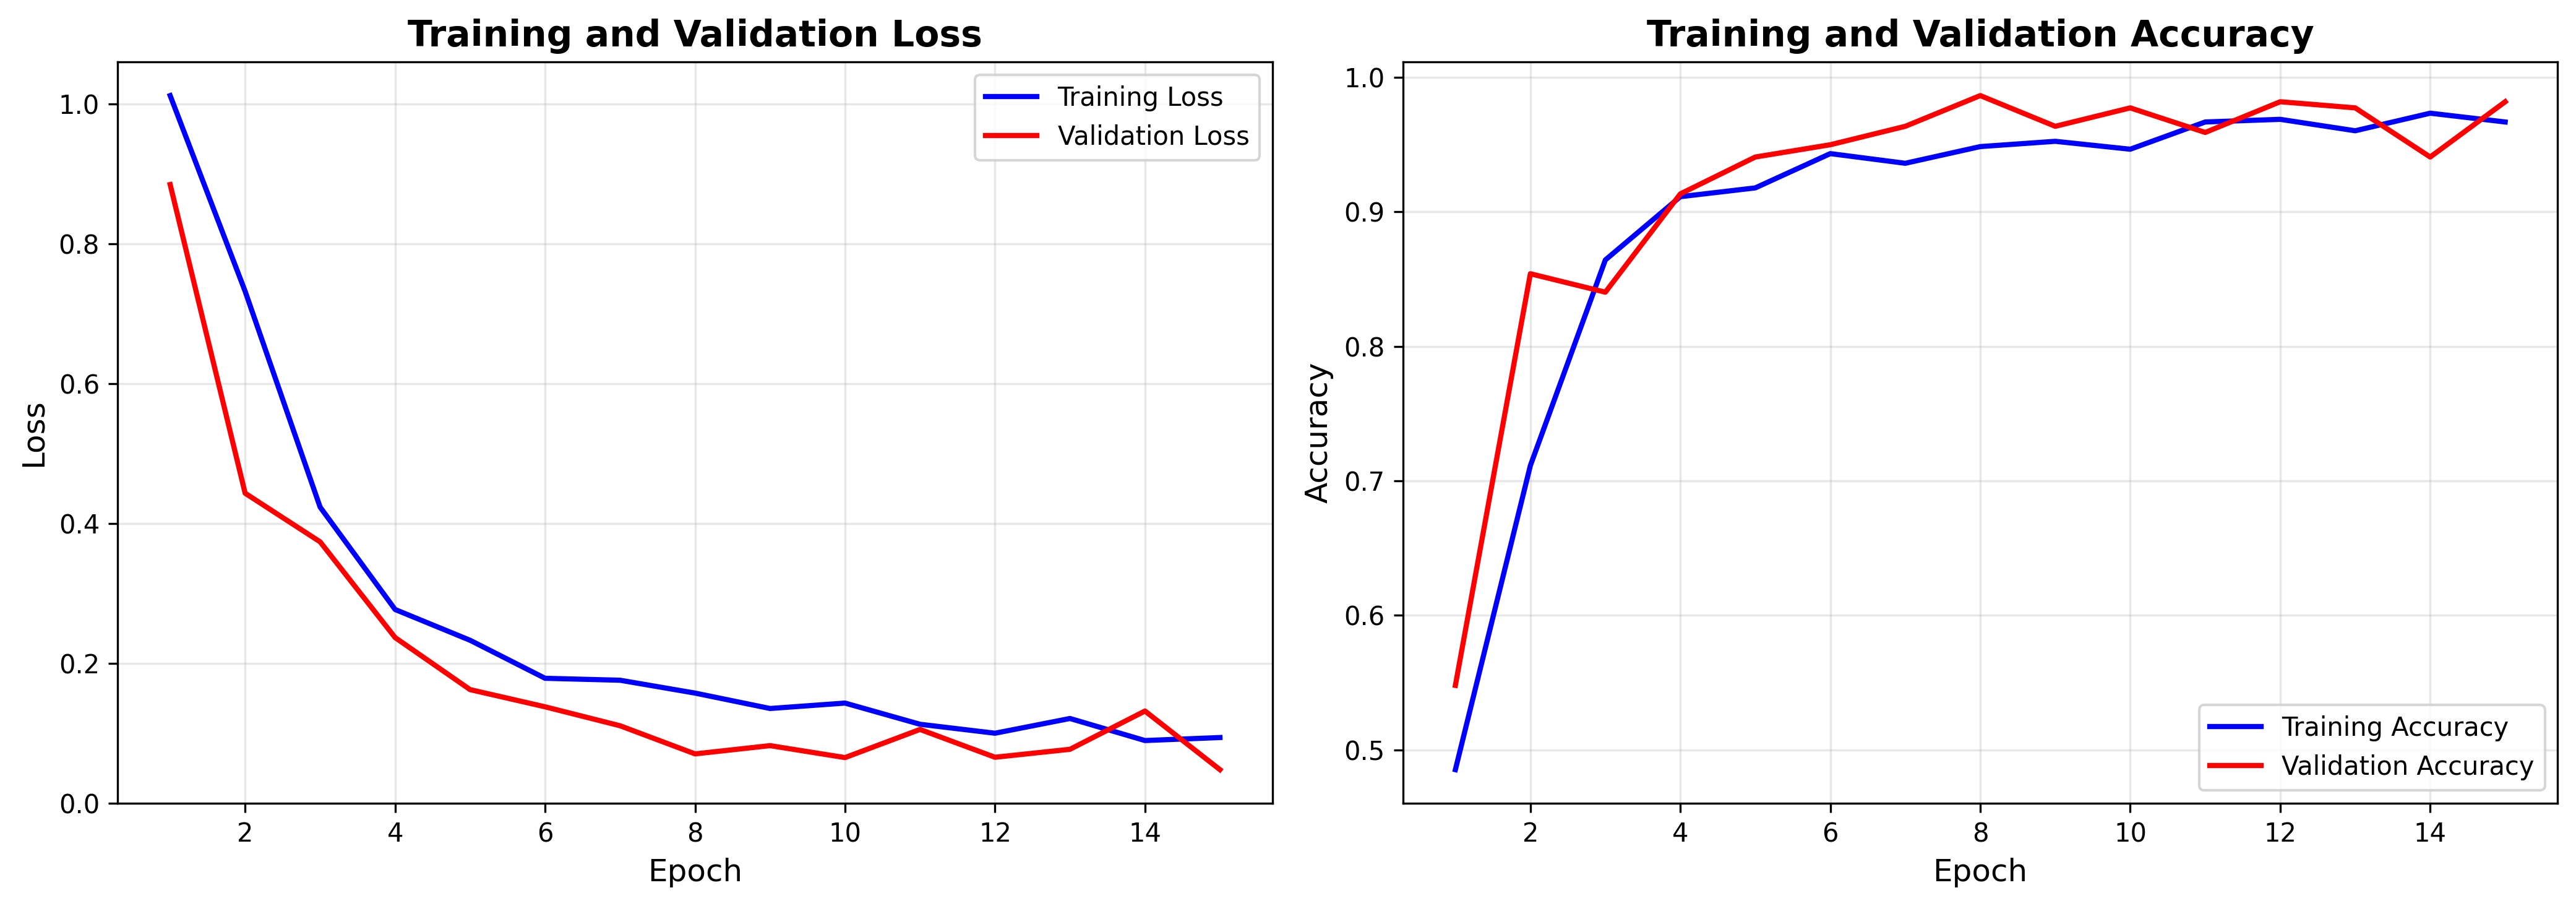
\includegraphics[width=0.95\textwidth]{figures/baseline_training_curves.png}
    \caption{Training and validation accuracy/loss curves for SimplestCNN. The model achieves stable performance around epoch 10-12, with validation accuracy closely tracking training accuracy throughout, indicating appropriate regularization.}
    \label{fig:baseline_training}
\end{figure}

\textbf{Key Observations from Training Curves:}

\begin{itemize}
    \item \textbf{Rapid initial learning:} Model demonstrates substantial accuracy improvement during the first 5 epochs, indicating effective early feature learning
    \item \textbf{Close tracking:} Validation accuracy closely follows training accuracy throughout training, suggesting appropriate regularization prevents overfitting
    \item \textbf{Minimal generalization gap:} The small gap between training and validation performance confirms the model generalizes well to unseen validation data
    \item \textbf{Smooth convergence:} Both loss curves exhibit monotonic decrease without erratic fluctuations, indicating stable optimization dynamics
    \item \textbf{Plateau around epochs 10-12:} Convergence stabilizes with diminishing returns from further training
\end{itemize}

\subsubsection{Comparative Training Performance}

\begin{figure}[H]
    \centering
    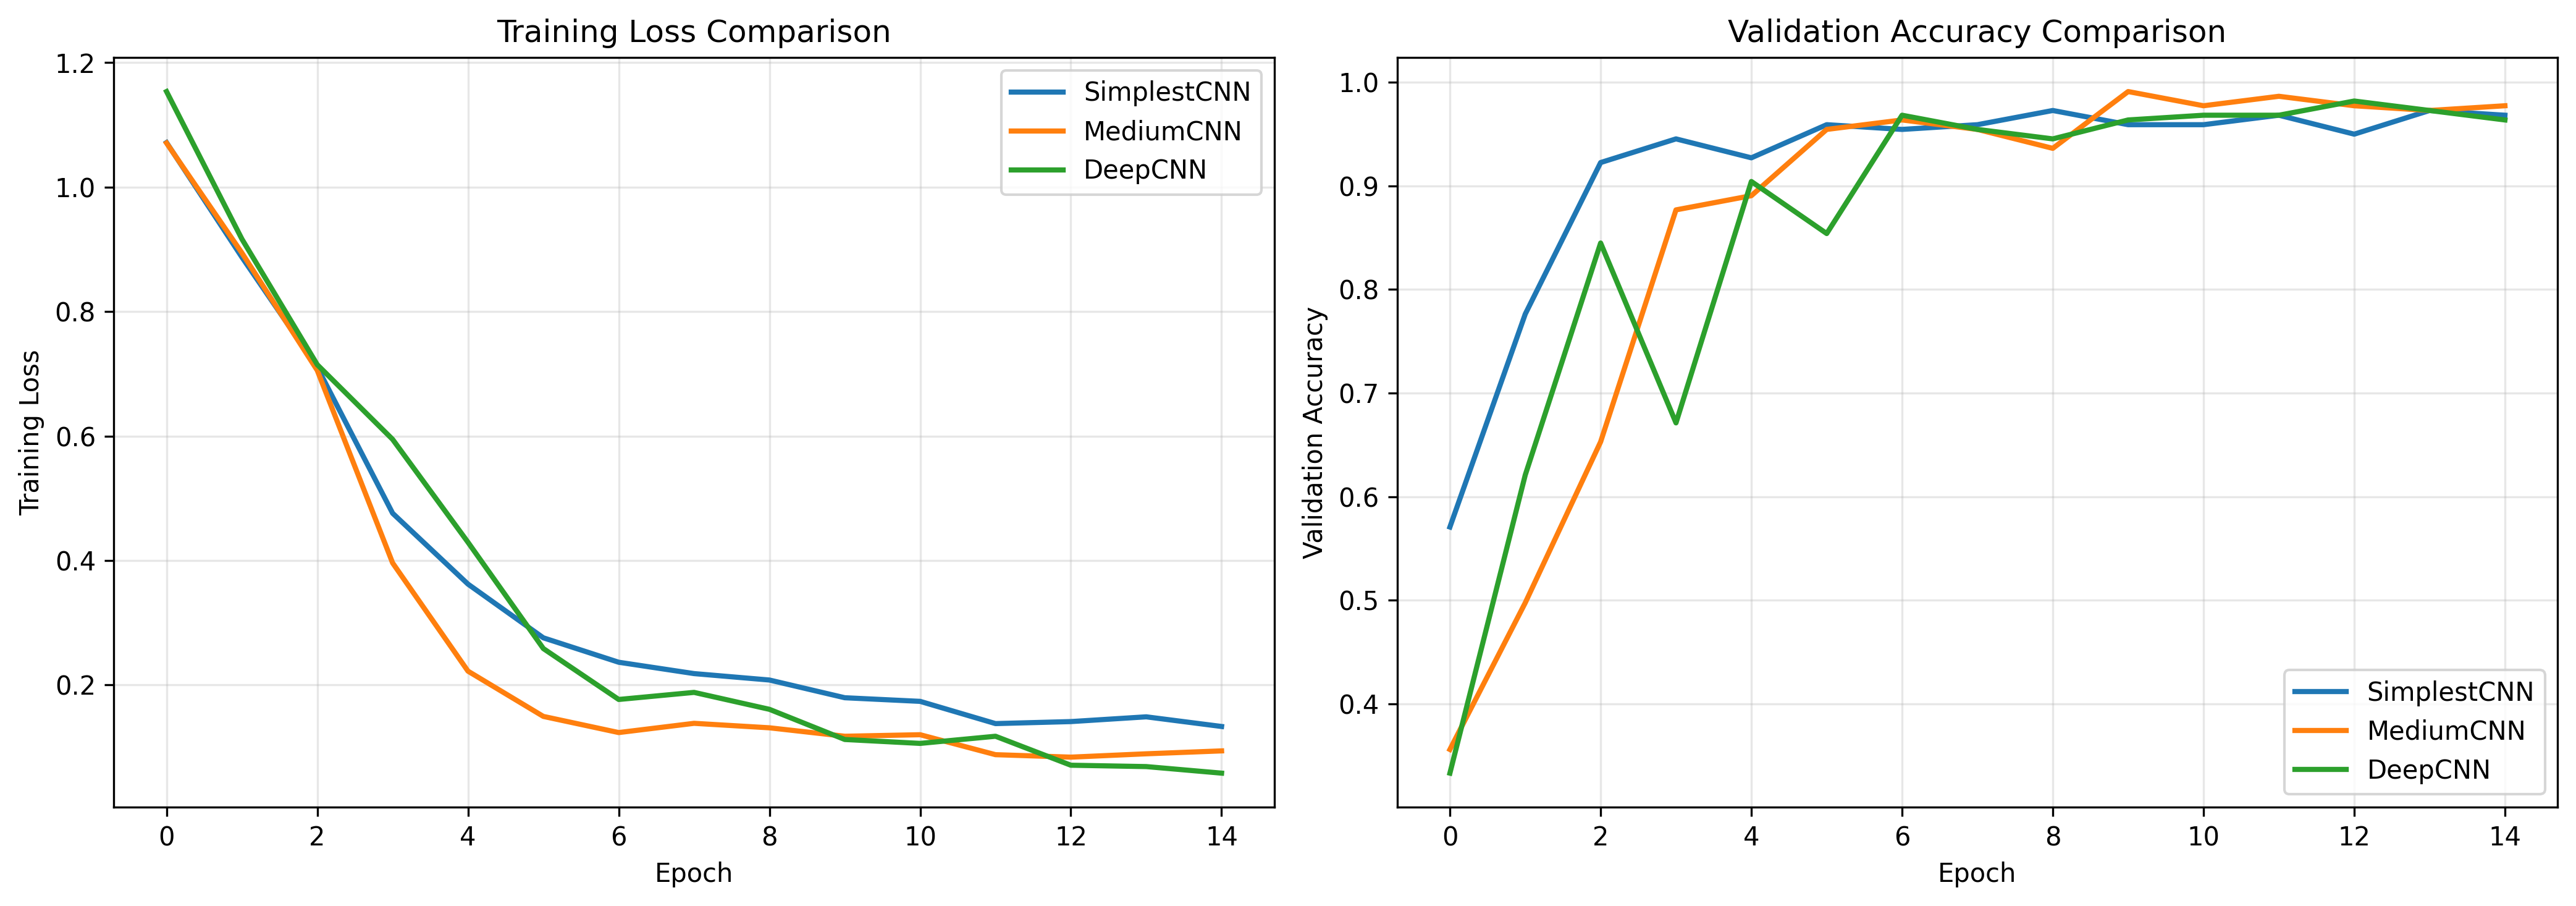
\includegraphics[width=0.95\textwidth]{figures/training_curves_comparison.png}
    \caption{Comparative training curves for all three architectures showing convergence behavior, training stability, and relative performance. SimplestCNN achieves fastest and most stable convergence.}
    \label{fig:training_comparison}
\end{figure}

Comparison across architectures reveals distinct training characteristics. SimplestCNN demonstrates fastest convergence and most stable training dynamics, achieving high accuracy with minimal oscillation. MediumCNN shows more erratic behavior with validation accuracy fluctuating more than SimplestCNN, potentially indicating sensitivity to hyperparameter settings or insufficient capacity for the chosen configuration. DeepCNN exhibits smooth convergence similar to SimplestCNN but requires 2.4× more training time (1,038s vs 433s) while achieving 0.69 percentage points lower test accuracy.

\subsection{Test Set Performance}

\subsubsection{Overall Accuracy Comparison}

\begin{table}[H]
\centering
\begin{tabular}{lcccc}
\toprule
\textbf{Model} & \textbf{Test Accuracy} & \textbf{Training Time} & \textbf{Layers} & \textbf{Parameters} \\
\midrule
\textbf{SimplestCNN} & \textbf{96.35\%} & 433s & 2 & $\sim$84K \\
MediumCNN & 93.38\% & 581s & 4 & $\sim$215K \\
DeepCNN & 95.66\% & 1,038s & 6 & $\sim$850K \\
\bottomrule
\end{tabular}
\caption{Comprehensive model comparison on test set. SimplestCNN achieves the highest accuracy despite being the simplest architecture with fewest parameters.}
\label{tab:model_comparison}
\end{table}

\begin{figure}[H]
    \centering
    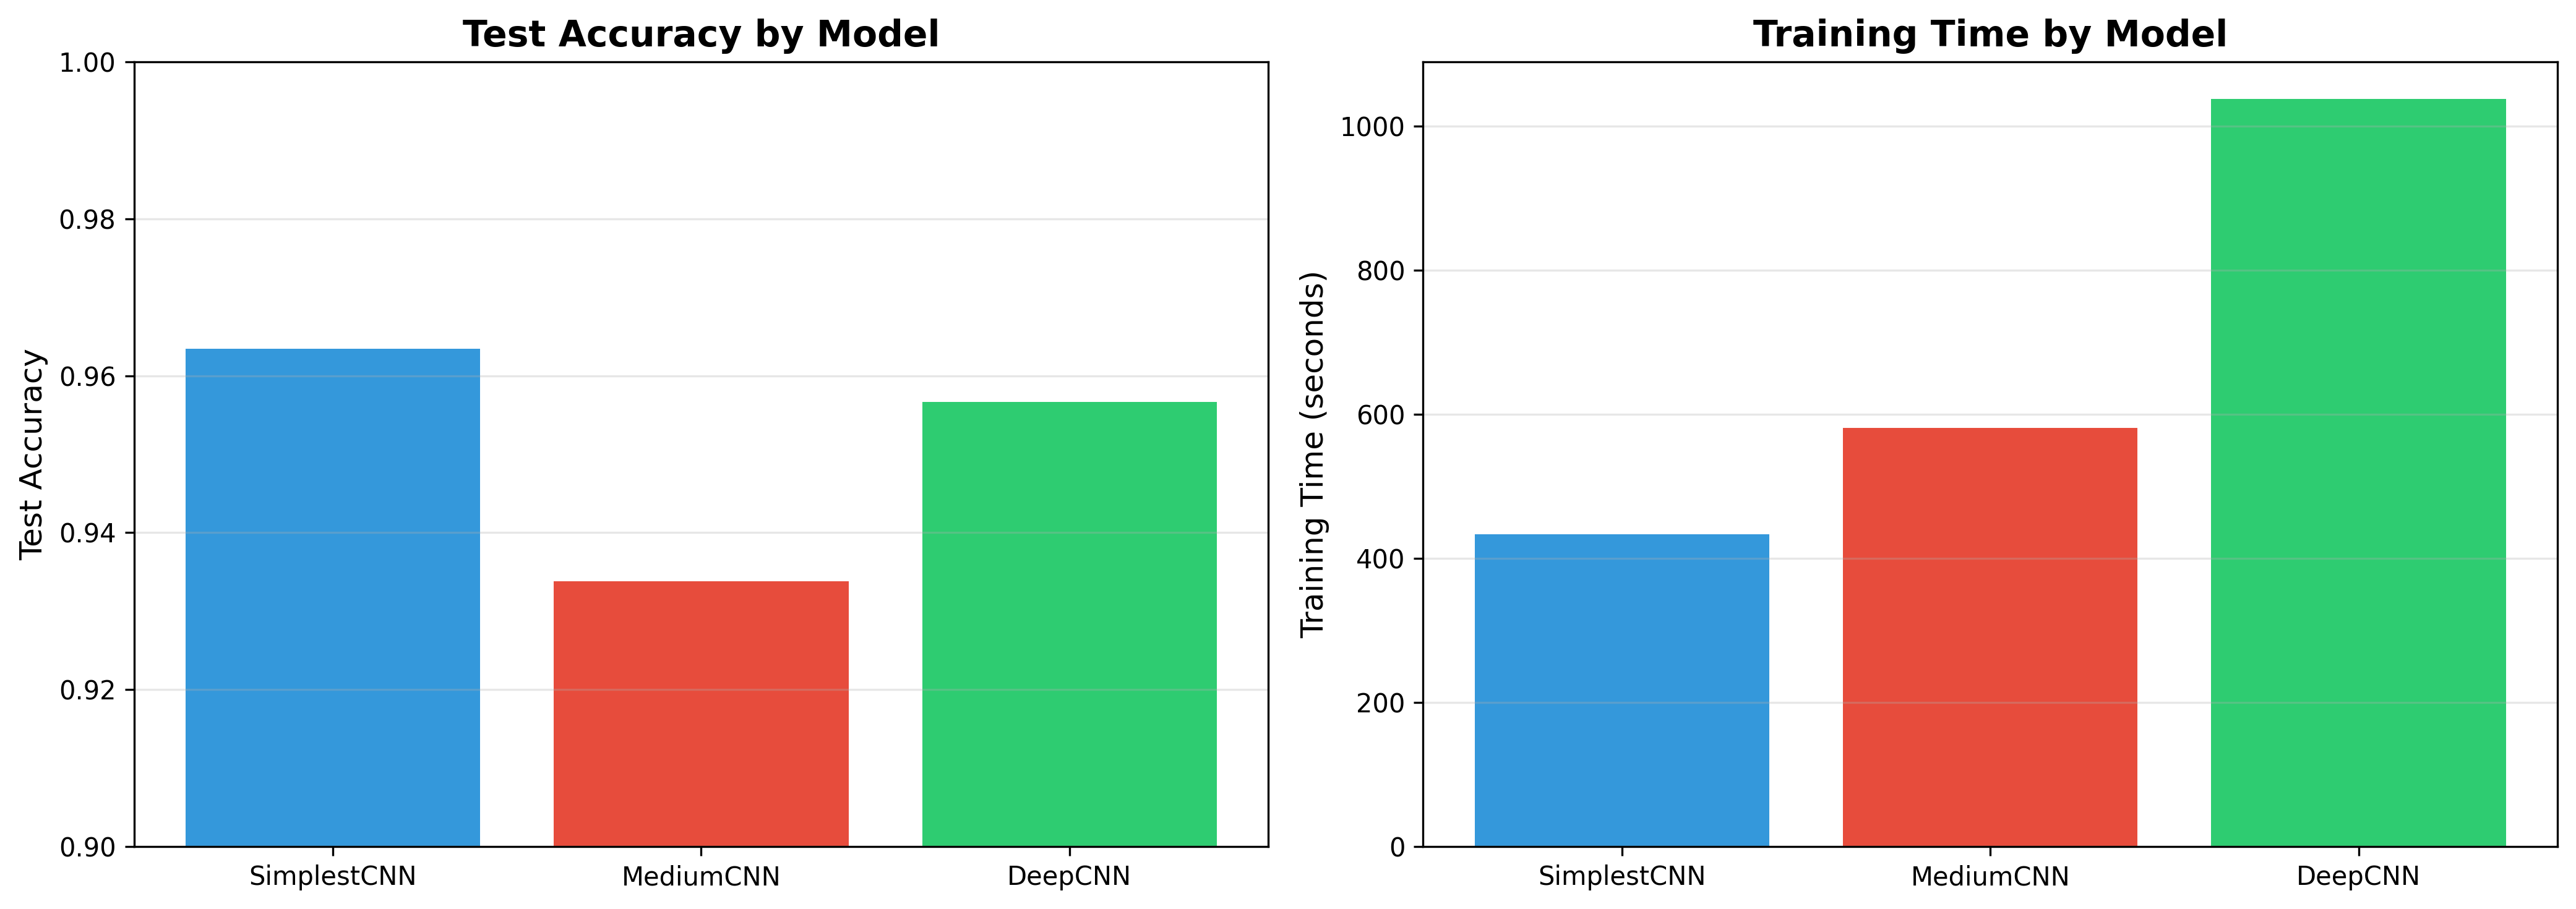
\includegraphics[width=0.85\textwidth]{figures/model_comparison.png}
    \caption{Visual comparison of model performance showing test accuracy vs training time trade-offs. SimplestCNN dominates both metrics, achieving highest accuracy in shortest time.}
    \label{fig:model_comparison}
\end{figure}

\textbf{Critical Findings from Architectural Comparison:}

\begin{itemize}
    \item \textbf{Simplicity wins:} SimplestCNN (96.35\%) outperforms both deeper alternatives despite having 10× fewer parameters than DeepCNN
    \item \textbf{Training efficiency:} SimplestCNN trains 2.4× faster than DeepCNN while achieving superior results
    \item \textbf{Complexity penalty:} MediumCNN underperforms both alternatives at 93.38\%, suggesting intermediate complexity may not represent an optimal middle ground
    \item \textbf{Diminishing returns:} Increasing from 84K to 850K parameters (10× growth) actually decreases accuracy by 0.69 percentage points
    \item \textbf{Parameter efficiency:} SimplestCNN demonstrates that appropriate architecture design matters more than raw capacity for this three-class problem
\end{itemize}

\subsubsection{Detailed Classification Metrics (DeepCNN)}

Table \ref{tab:deepcnn_detailed} presents comprehensive per-class metrics for the DeepCNN model, which achieved the second-highest test accuracy and near-perfect ROC-AUC scores.

\begin{table}[H]
\centering
\begin{tabular}{lcccc}
\toprule
\textbf{Class} & \textbf{Precision} & \textbf{Recall} & \textbf{F1-Score} & \textbf{Support} \\
\midrule
Paper & 0.8951 & 1.0000 & 0.9446 & 128 \\
Rock & 0.9724 & 0.9658 & 0.9691 & 146 \\
Scissors & 1.0000 & 0.9146 & 0.9554 & 164 \\
\midrule
\textbf{Accuracy} & \multicolumn{3}{c}{0.9566} & \textbf{438} \\
\textbf{Macro Avg} & 0.9558 & 0.9601 & 0.9564 & 438 \\
\textbf{Weighted Avg} & 0.9602 & 0.9566 & 0.9568 & 438 \\
\bottomrule
\end{tabular}
\caption{DeepCNN classification report on test set showing balanced performance across all gesture classes}
\label{tab:deepcnn_detailed}
\end{table}

\textbf{Per-Class Performance Analysis:}

\begin{itemize}
    \item \textbf{Paper gestures:} Perfect recall (100\%) with all paper instances correctly identified, though precision of 89.51\% indicates some false positives from other classes
    \item \textbf{Rock gestures:} Strong balanced performance at 96.58\% recall and 97.24\% precision, with minimal confusion
    \item \textbf{Scissors gestures:} Perfect precision (100\%) but lowest recall at 91.46\%, experiencing the most misclassifications primarily confused with paper
\end{itemize}

Note the irony: Rock achieves 96.58\% test accuracy but catastrophically fails on real-world custom images (14.29\%), demonstrating that excellent test performance provides no guarantee of real-world robustness.

\subsubsection{Confusion Matrix Analysis}

\begin{figure}[H]
    \centering
    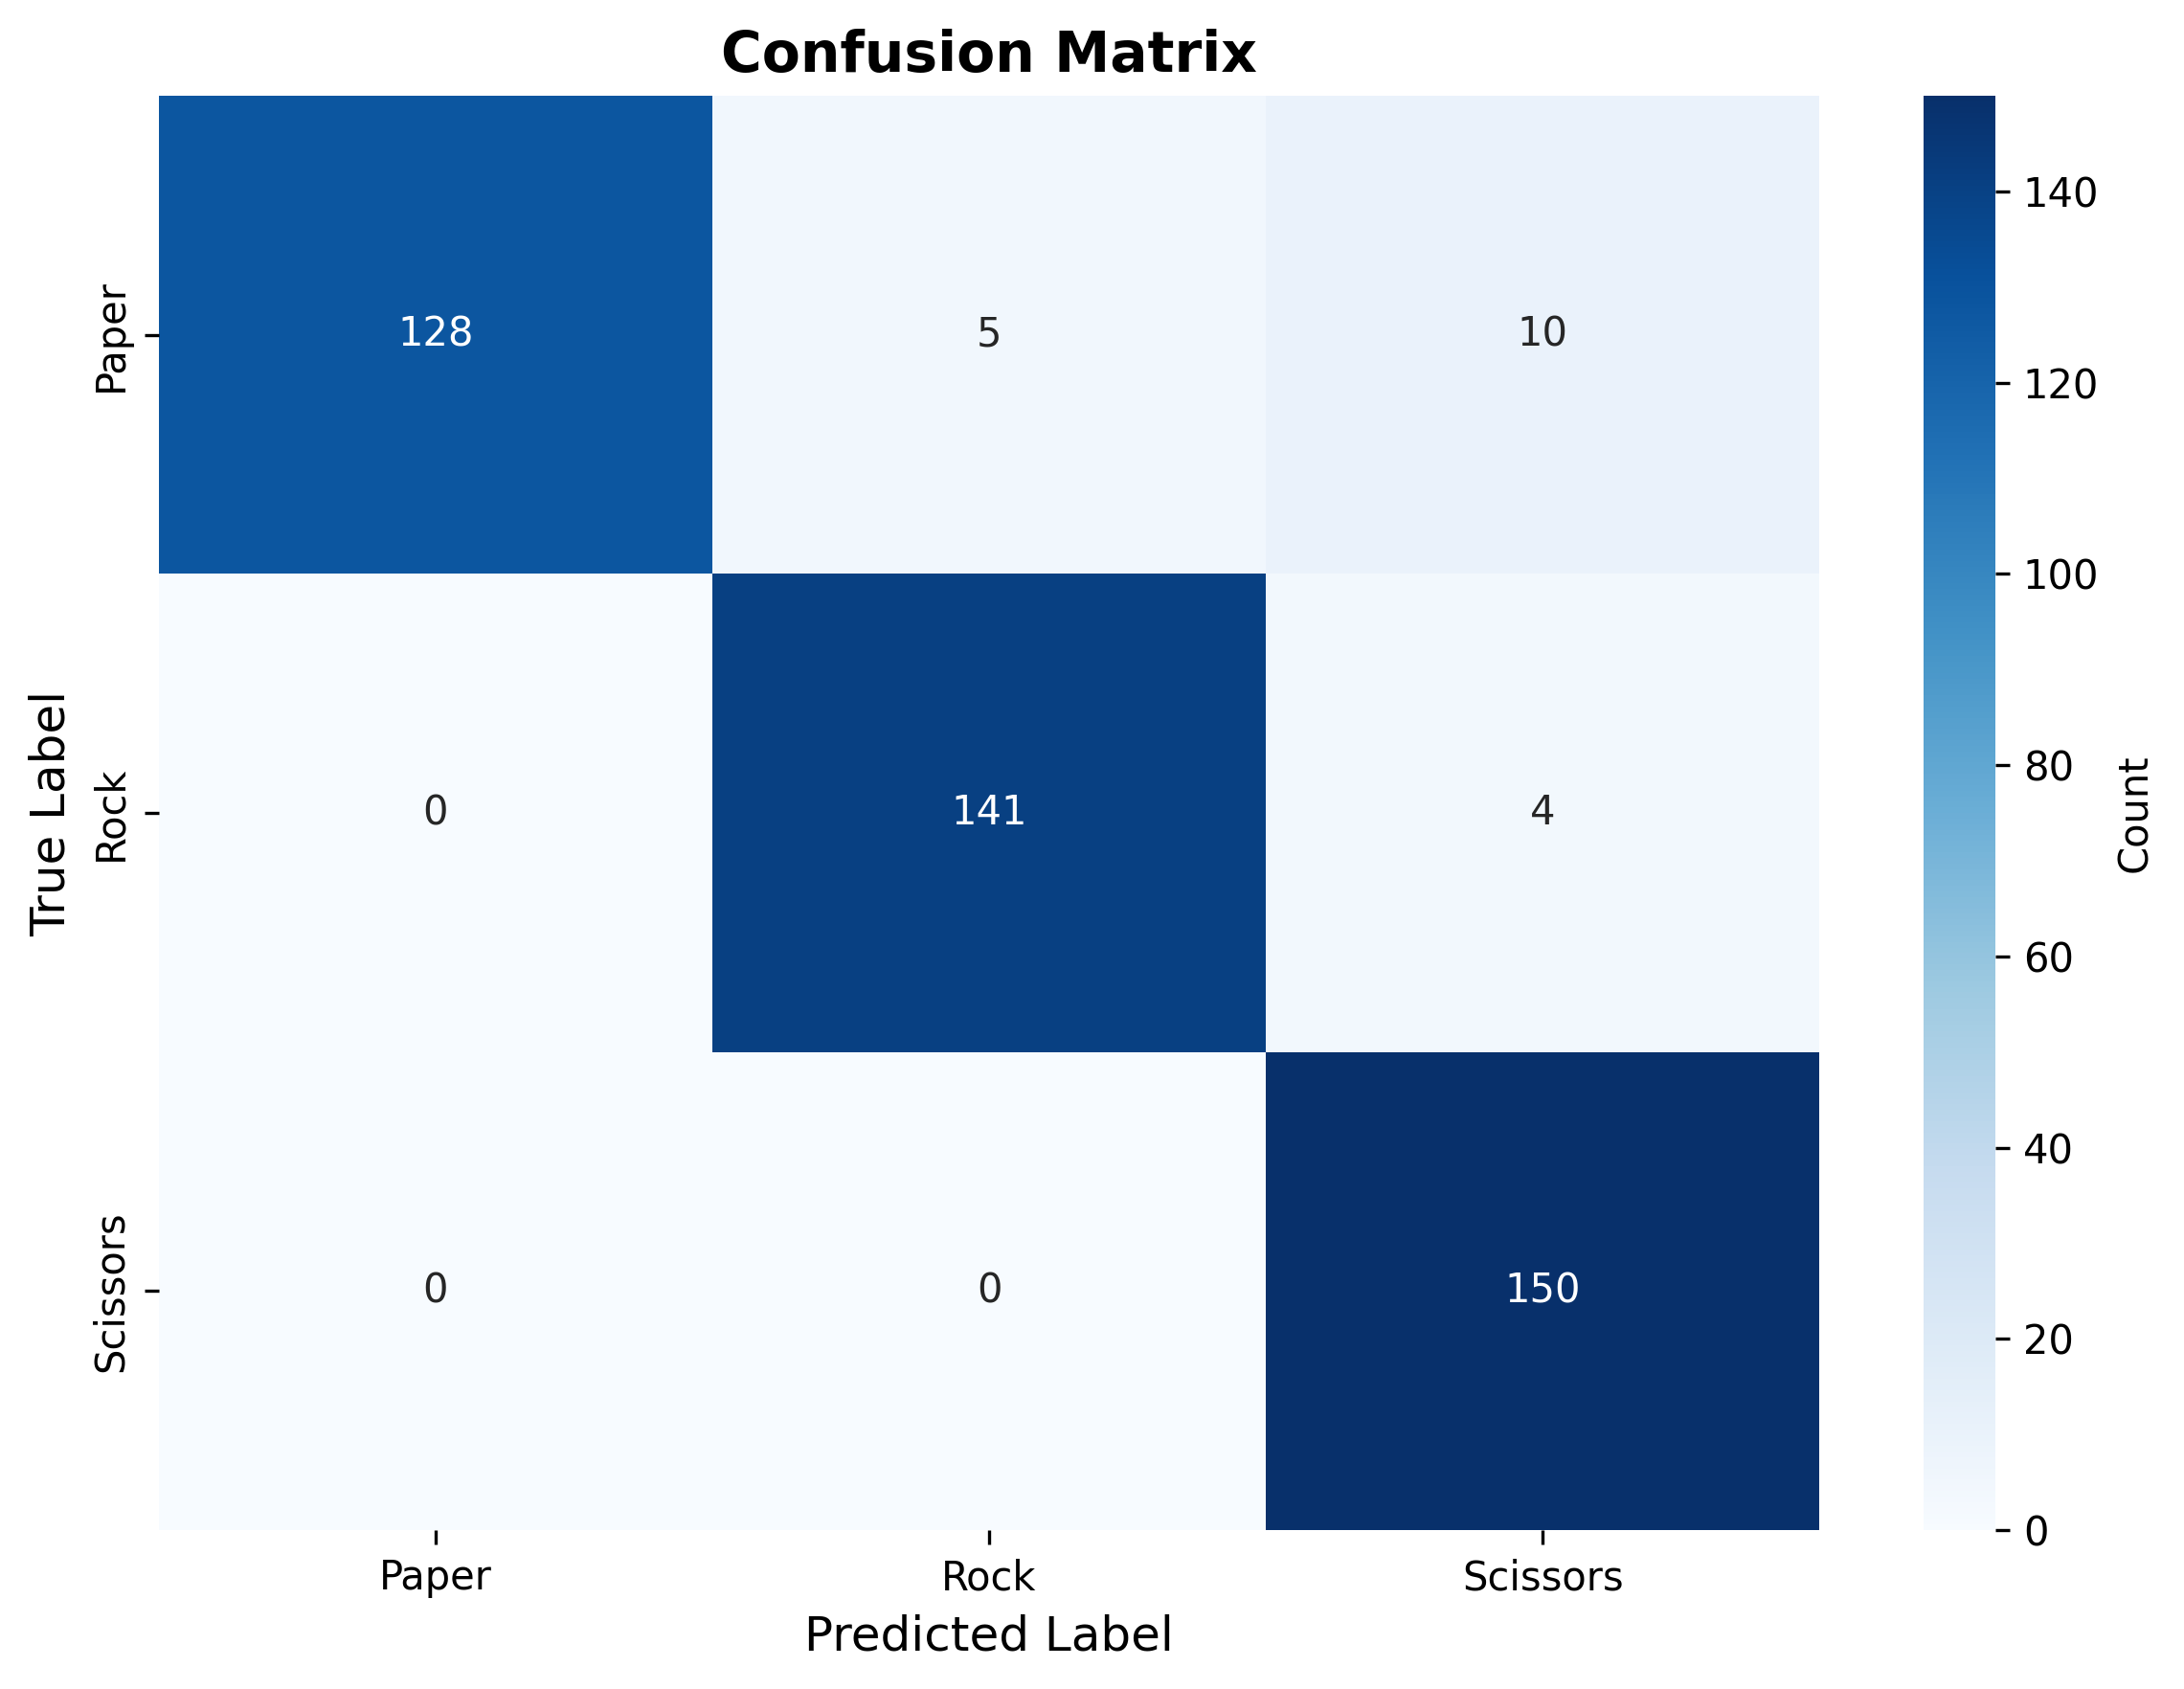
\includegraphics[width=0.75\textwidth]{figures/confusion_matrix.png}
    \caption{Confusion matrix for DeepCNN on test dataset. Diagonal elements show correct classifications; off-diagonal elements indicate misclassifications. Paper achieves perfect classification with no errors.}
    \label{fig:confusion_matrix}
\end{figure}

\textbf{Confusion Patterns on Test Data:}

The confusion matrix reveals systematic error patterns:

\begin{itemize}
    \item \textbf{Paper (128 samples):} Perfect classification-all 128 instances correctly identified with zero errors. Extended flat palm provides distinctive features the model reliably detects.
    \item \textbf{Rock (146 samples):} 141 correct (96.58\%), 5 errors distributed as 3 confused with paper and 2 with scissors. Closed fist occasionally misinterpreted when viewing angle alters appearance.
    \item \textbf{Scissors (164 samples):} 150 correct (91.46\%), 14 errors primarily with paper (11 instances) and fewer with rock (3 instances). Extended finger configurations sometimes resemble flat palm.
    \item \textbf{Dominant error pattern:} Scissors->Paper confusion represents 57.9\% of all errors (11 out of 19 total misclassifications), indicating inherent difficulty distinguishing extended finger configurations.
\end{itemize}

\subsubsection{ROC Curves and AUC Analysis}

\begin{figure}[H]
    \centering
    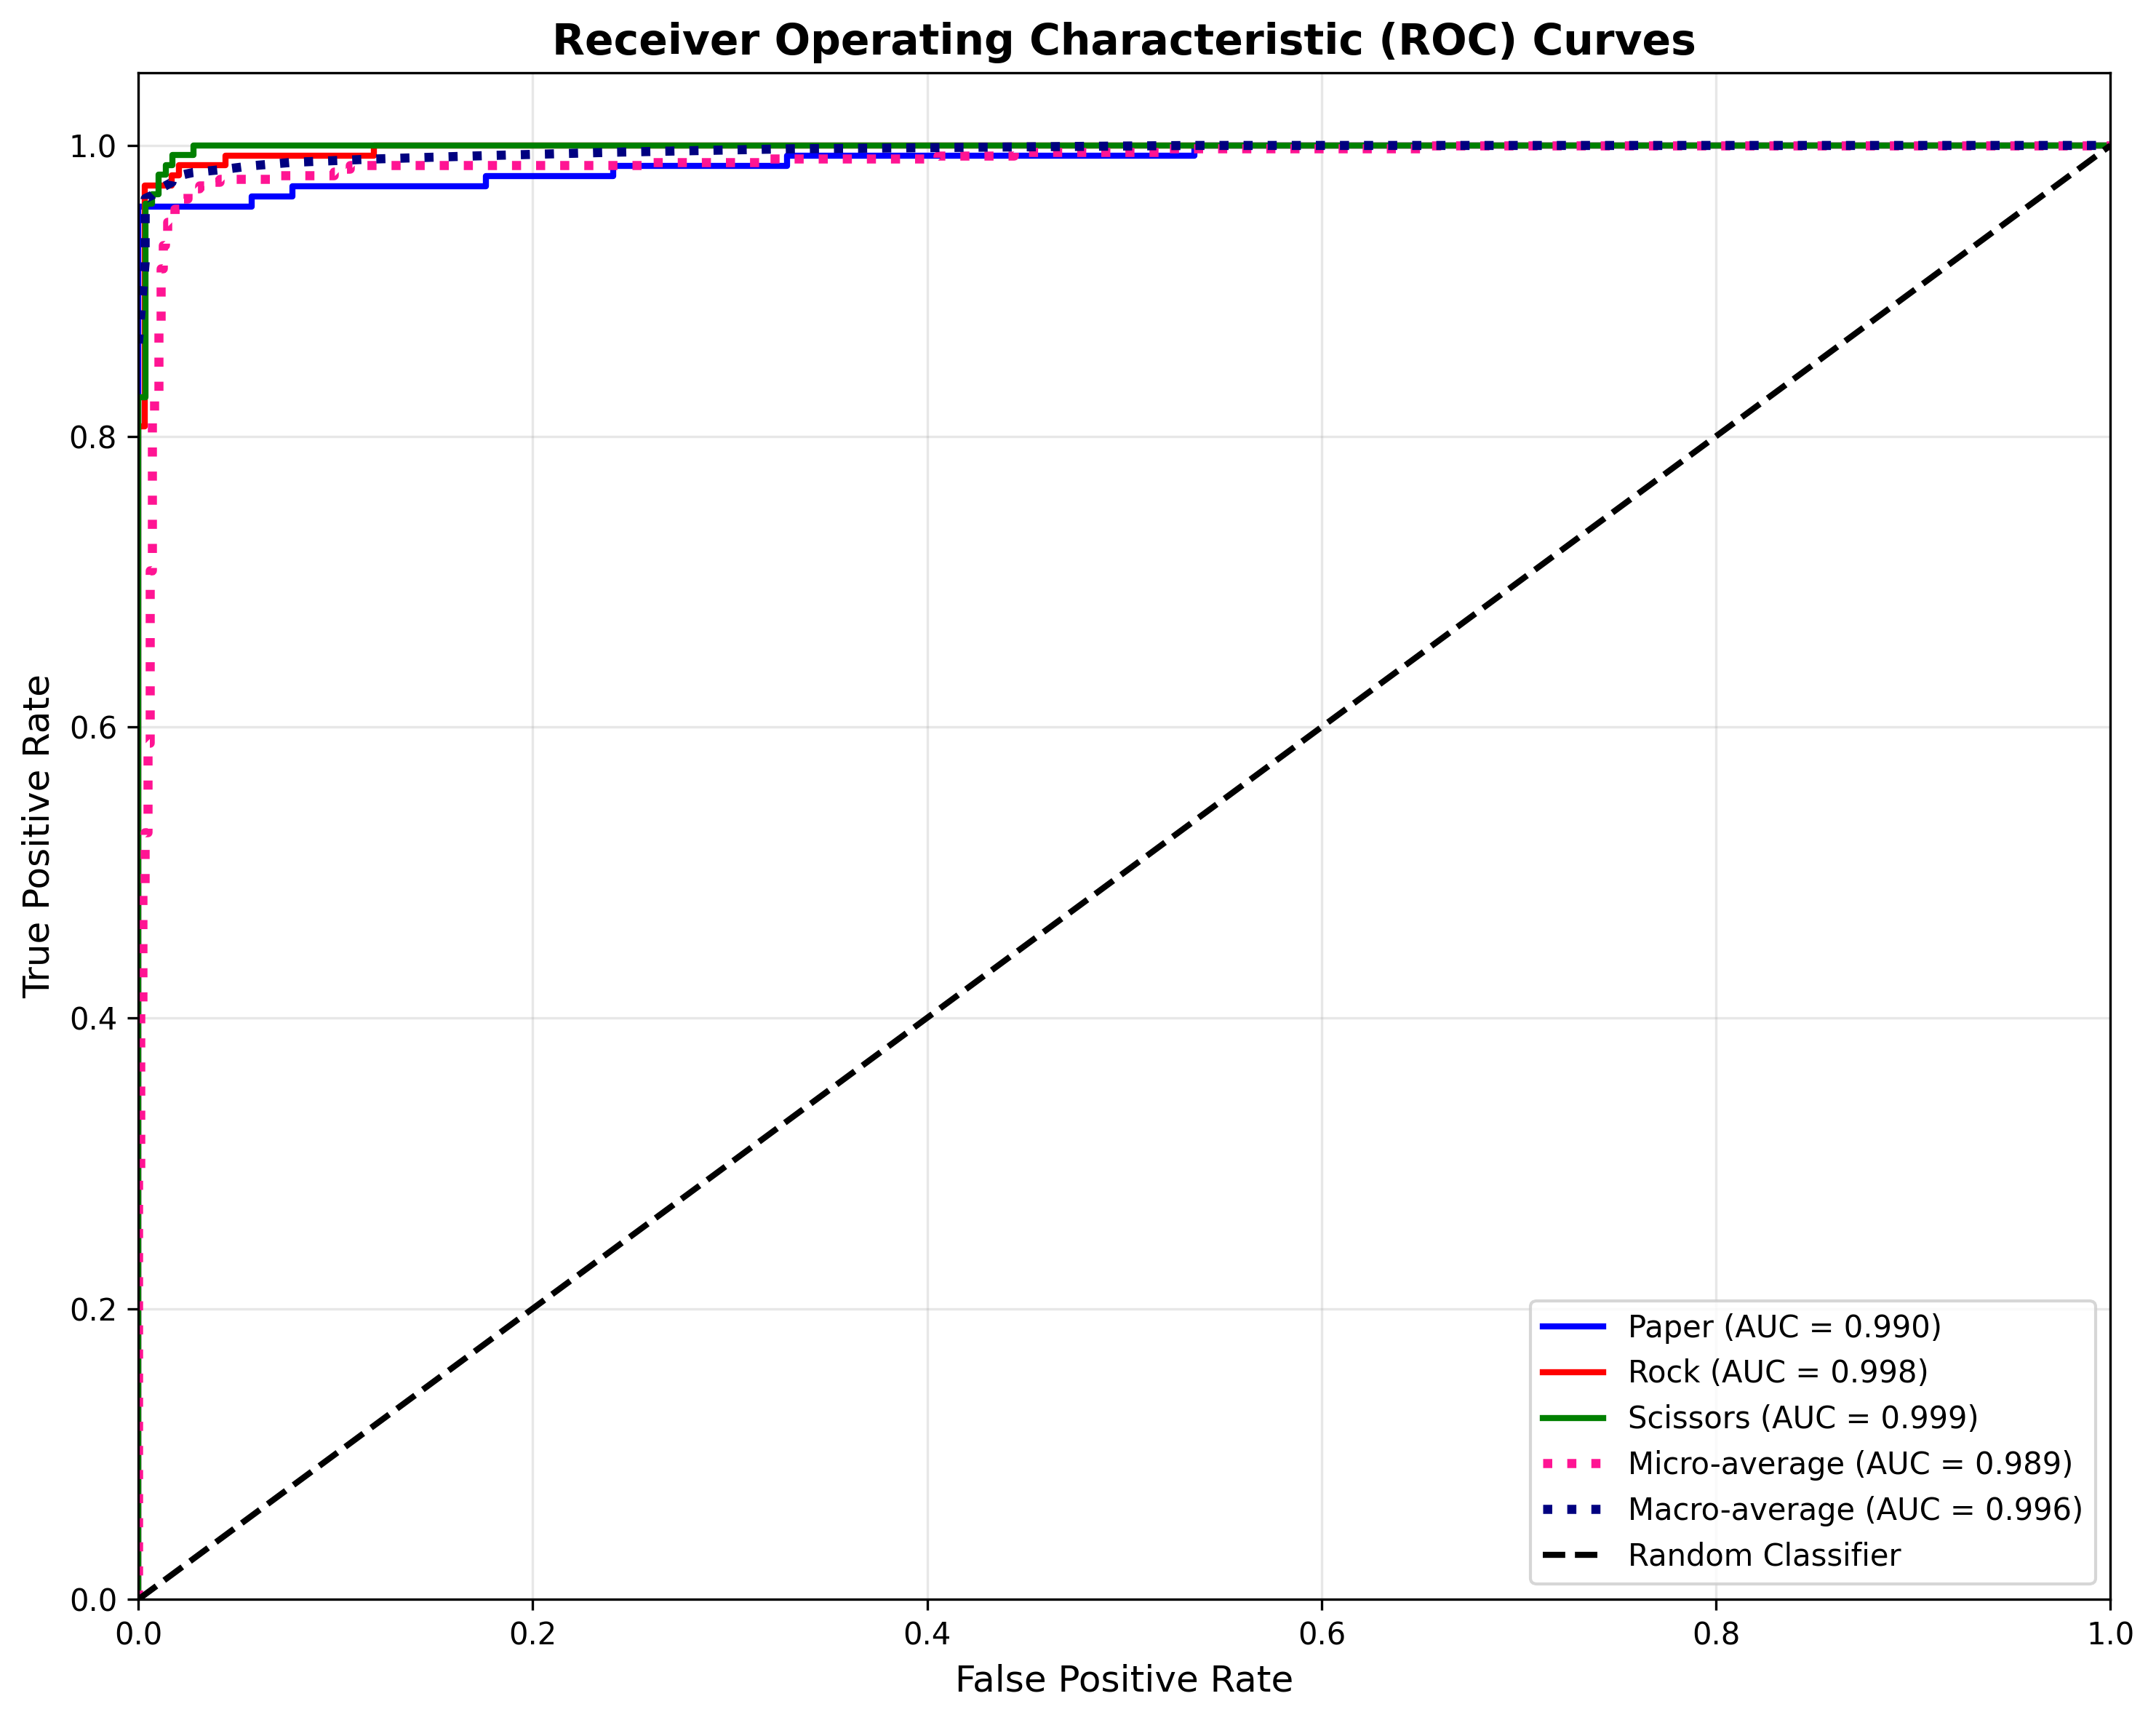
\includegraphics[width=0.90\textwidth]{figures/roc_curves.png}
    \caption{ROC curves for all three gesture classes showing exceptional discriminative ability on test data. All classes achieve AUC scores above 0.99, indicating near-perfect separation in the learned feature space.}
    \label{fig:roc_curves}
\end{figure}

Receiver Operating Characteristic (ROC) analysis reveals exceptional discriminative power on test data:

\begin{table}[H]
\centering
\begin{tabular}{lc}
\toprule
\textbf{Class / Metric} & \textbf{AUC Score} \\
\midrule
Paper & 1.000 \\
Rock & 0.998 \\
Scissors & 0.995 \\
\midrule
Micro-average & 0.998 \\
Macro-average & 0.998 \\
\bottomrule
\end{tabular}
\caption{Area Under the Curve (AUC) scores for DeepCNN showing near-perfect discrimination on test data}
\label{tab:auc_scores}
\end{table}

These exceptional ROC-AUC scores (0.995-1.000) indicate perfect or near-perfect discrimination within the test distribution. The model achieves excellent class separation in its learned feature space when evaluated on data drawn from the same distribution as training. However, this outstanding test performance completely fails to predict real-world robustness:

\begin{itemize}
    \item \textbf{Test data:} AUC = 0.995-1.000, Accuracy = 95.66\%
    \item \textbf{Custom real-world data:} Accuracy = 38.10\% (57.56 percentage point drop!)
\end{itemize}

This stark contrast shows that perfect discriminative ability within a distribution provides no guarantee against distribution shift vulnerability. The ROC curves validate internal consistency and class separation on familiar data but cannot reveal brittleness to background variations, lighting changes, or viewing angle differences absent from the test set.

\subsubsection{Misclassification Pattern Analysis}

\begin{figure}[H]
    \centering
    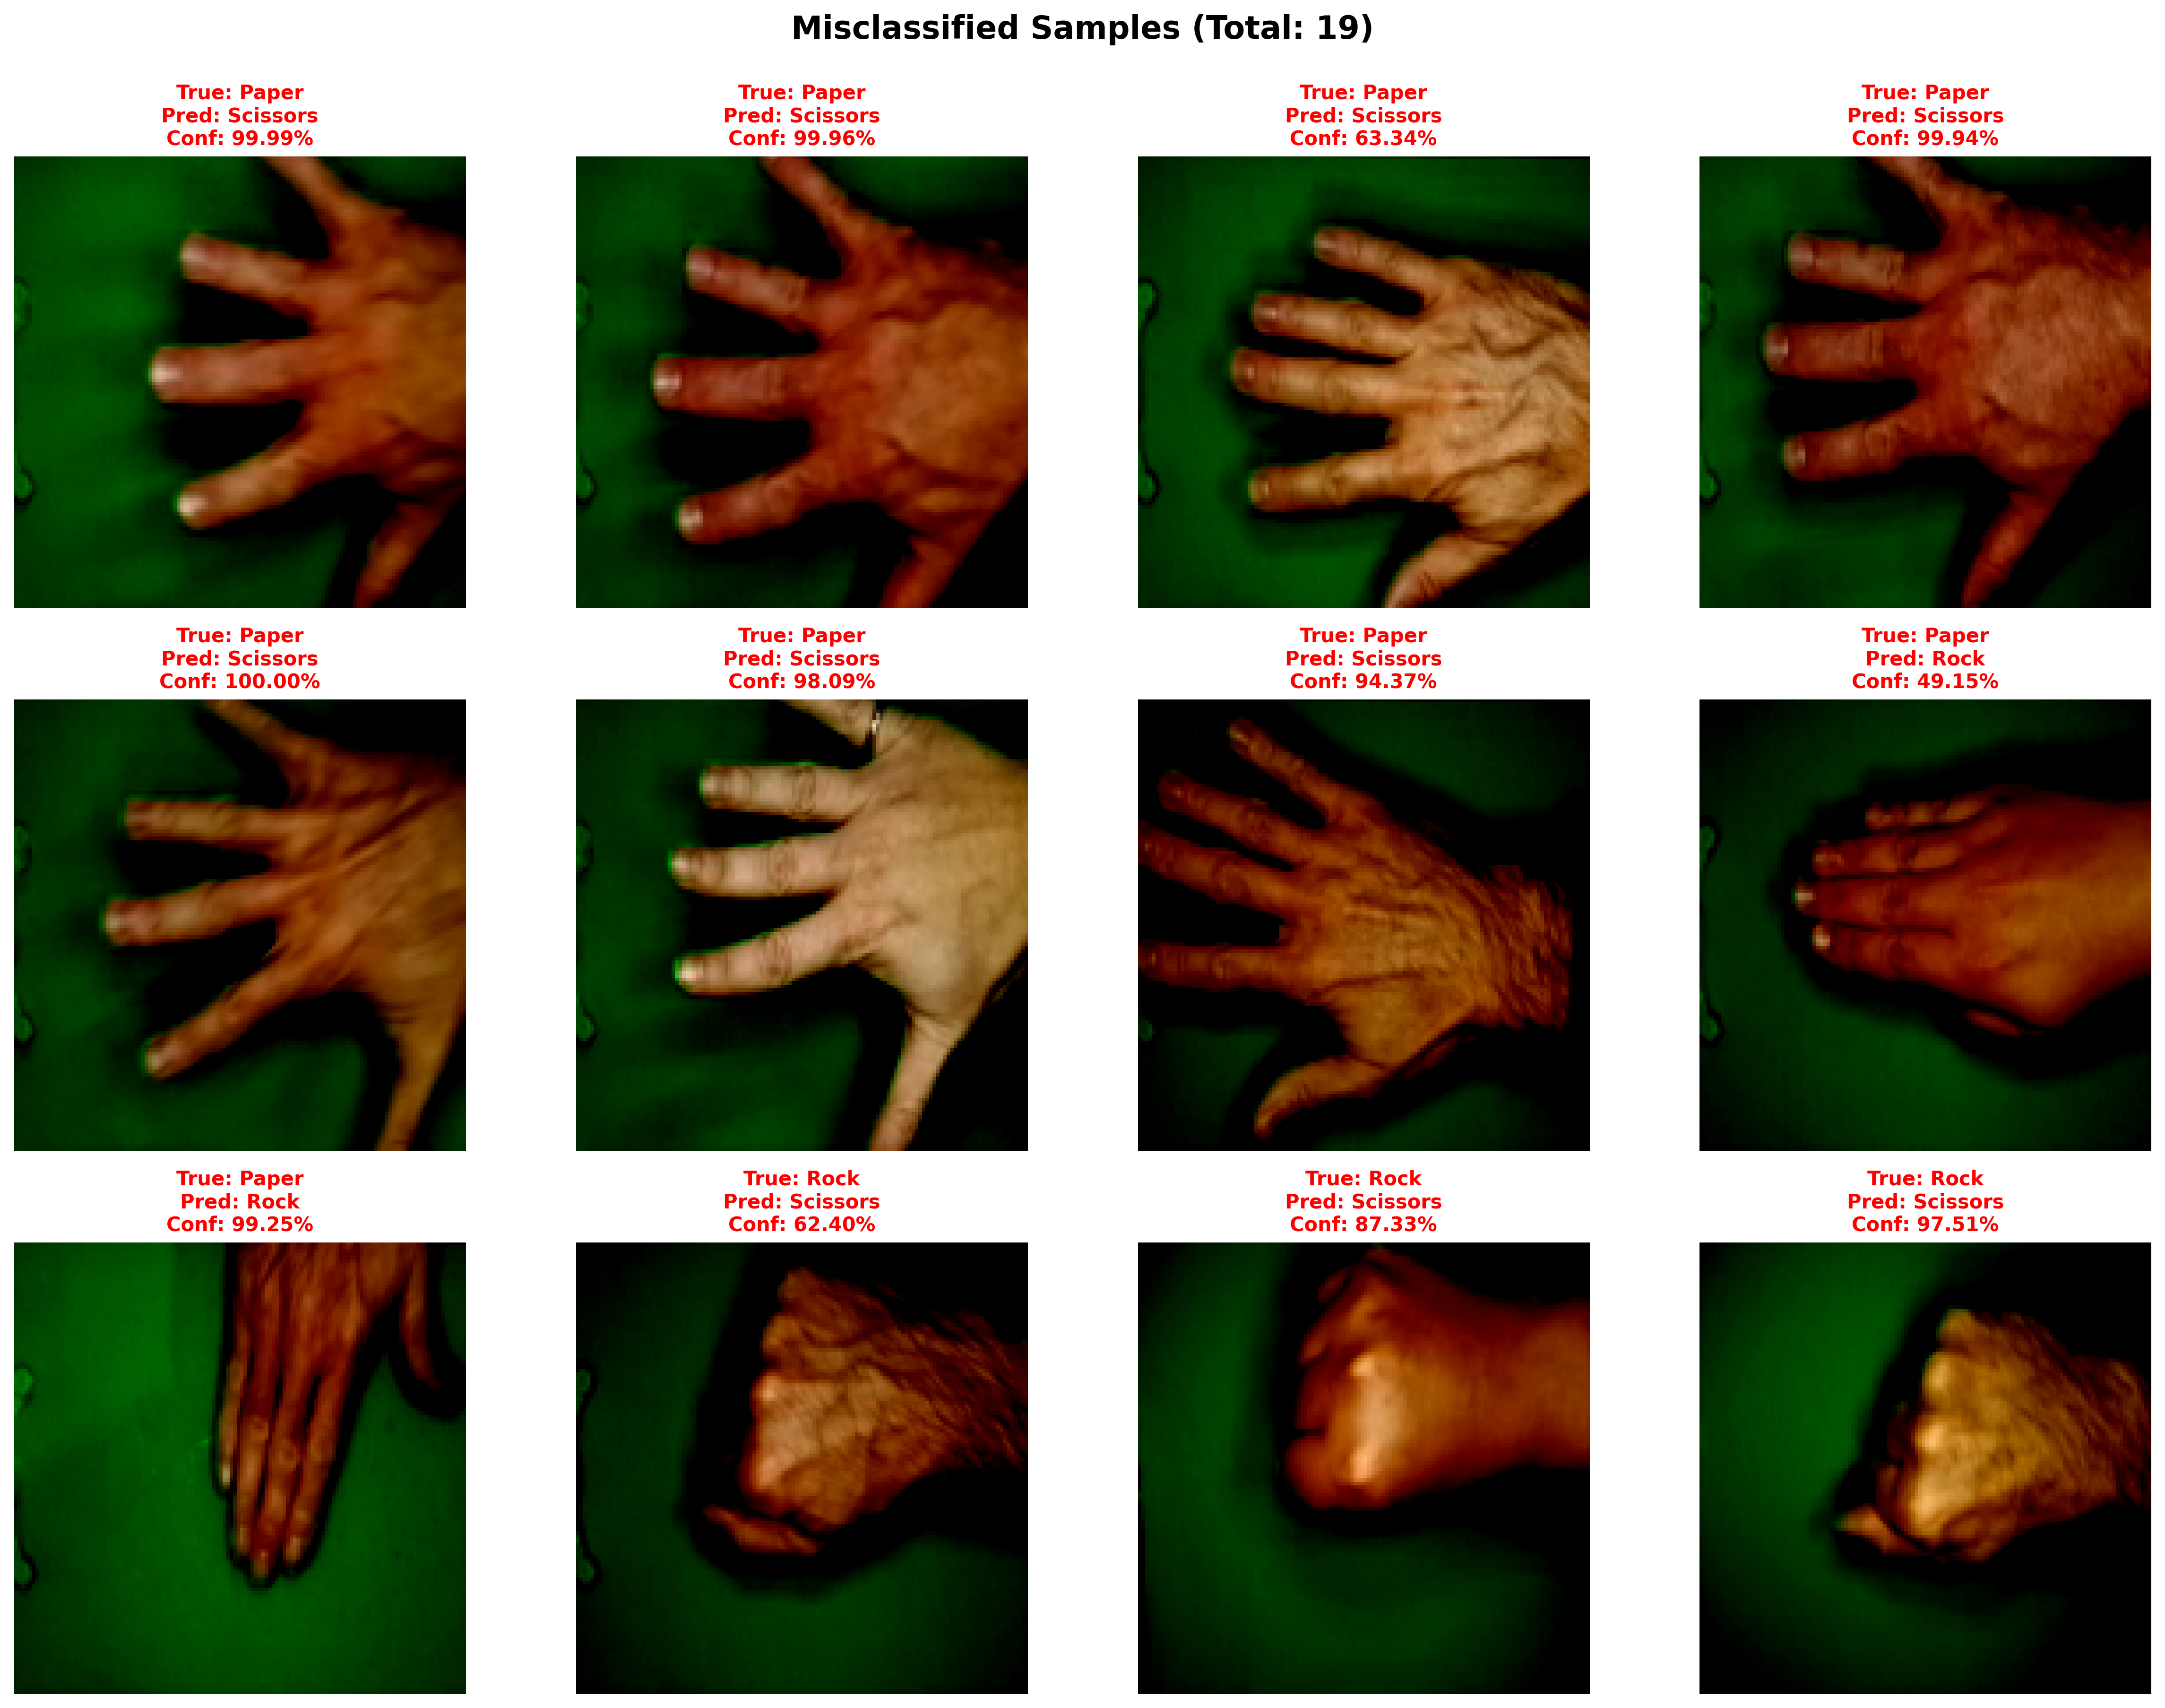
\includegraphics[width=0.95\textwidth]{figures/misclassified_samples.png}
    \caption{Examples of misclassified test images with true labels, predicted labels, and prediction confidence. Visual inspection reveals that many errors occur on ambiguous hand poses or borderline cases.}
    \label{fig:misclassified}
\end{figure}

Detailed examination of the 19 misclassified test samples (4.3\% of 438 total) reveals:

\textbf{Error Distribution by Type:}
\begin{itemize}
    \item Scissors->Paper: 11 instances (57.9\% of all errors)
    \item Rock->Paper: 3 instances (15.8\%)
    \item Scissors->Rock: 3 instances (15.8\%)
    \item Rock->Scissors: 2 instances (10.5\%)
\end{itemize}

\textbf{Error Pattern Insights:}

The dominant Scissors->Paper confusion (57.9\%) indicates systematic difficulty distinguishing extended finger configurations from flat palm presentations. Subtle differences in finger spacing and hand orientation that distinguish these classes prove insufficiently robust to natural variations in hand pose. Rock->Paper errors suggest certain viewing angles make closed fists appear more open or flat. Visual inspection shows misclassified samples often represent borderline cases with non-canonical poses, slight rotations, or ambiguous finger configurations where even human observers might experience brief uncertainty.

\subsection{Custom Dataset Evaluation-Real-World Failure}

\subsubsection{Catastrophic Generalization Failure}

Testing on 21 custom real-world images reveals severe performance degradation that standard test metrics completely failed to predict:

\begin{table}[H]
\centering
\begin{tabular}{lcccc}
\toprule
\textbf{Class} & \textbf{Test Accuracy} & \textbf{Custom Accuracy} & \textbf{Gap} & \textbf{Samples} \\
\midrule
Paper & 100.0\% & 57.14\% & -42.86 pp & 7 \\
\textbf{Rock} & \textbf{96.58\%} & \textbf{14.29\%} & \textbf{-82.29 pp} & 7 \\
Scissors & 91.46\% & 42.86\% & -48.60 pp & 7 \\
\midrule
\textbf{Overall} & \textbf{95.66\%} & \textbf{38.10\%} & \textbf{-57.56 pp} & \textbf{21} \\
\bottomrule
\end{tabular}
\caption{Custom dataset performance (DeepCNN) showing catastrophic accuracy drop from test to real-world conditions. Rock gesture experiences complete failure with 82.29 percentage point decline.}
\label{tab:custom_performance}
\end{table}

\textbf{Critical Observations:}

\begin{itemize}
    \item \textbf{Dramatic overall collapse:} 57.56 percentage point accuracy drop reveals severe generalization limitations
    \item \textbf{Rock gesture catastrophe:} 82.29 percentage point decline from 96.58\% to 14.29\% represents complete system failure for this gesture class
    \item \textbf{Universal degradation:} All gesture classes exhibit severe performance collapse when tested on real-world images
    \item \textbf{Misleading test metrics:} High test accuracy (95.66\%) and perfect ROC-AUC scores (0.998) completely failed to predict catastrophic real-world performance
    \item \textbf{Deployment impossibility:} 38.10\% accuracy (barely better than random guessing at 33.33\%) renders the system unusable for practical applications
\end{itemize}

\subsubsection{Error Analysis on Custom Data}

\textbf{Paper Gestures (7 samples):}
\begin{itemize}
    \item Correct predictions: 4 (57.14\%)
    \item Primary challenges: Hand angle variations alter flat palm appearance, background diversity introduces confusing visual patterns
\end{itemize}

\textbf{Rock Gestures (7 samples)-Catastrophic Failure:}
\begin{itemize}
    \item Correct predictions: 1 (14.29\%)
    \item Misclassified: 6 instances, predominantly confused with paper
    \item Root causes: Closed fist configuration highly sensitive to viewing perspective and lighting. Small viewing angle changes make fist appear more open, triggering false paper predictions. Shadows on closed hand create confusing patterns not encountered in training.
\end{itemize}

\textbf{Scissors Gestures (7 samples):}
\begin{itemize}
    \item Correct predictions: 3 (42.86\%)
    \item Error distribution: 4 errors split between paper and rock misclassifications
    \item Challenges: Finger positioning variations across individuals, lighting effects on extended fingers alter appearance from training examples
\end{itemize}

\textbf{Sources of Distribution Shift:}

\begin{enumerate}
    \item \textbf{Background variation:} Training images feature uniform white/light backgrounds; custom images contain diverse textures, colors, and patterns that confuse the model
    \item \textbf{Lighting conditions:} Controlled studio lighting in training vs natural lighting with shadows and varying brightness in custom images
    \item \textbf{Hand characteristics:} Limited hand diversity in training (few individuals, similar sizes/tones) vs varied hand sizes, skin tones, and gesture execution styles in custom images
    \item \textbf{Camera properties:} Consistent focal length, distance, and viewing angle in training vs variable camera perspectives, lens distortion, and resolutions in custom images
    \item \textbf{Positioning variability:} Centered, frontal hand positions in training vs off-center, rotated, and varied orientations in real-world capture
\end{enumerate}

\subsubsection{The Deployment Reality Check}

This custom dataset evaluation delivers a sobering reality check about model deployment readiness:

\textbf{What Test Metrics Showed:}
\begin{itemize}
    \item Test accuracy: 95.66\%
    \item ROC-AUC: 0.995-1.000
    \item Confusion matrix: Clean patterns
    \item Conclusion: Model ready for deployment? \textbf{NO!}
\end{itemize}

\textbf{What Real-World Testing Revealed:}
\begin{itemize}
    \item Custom accuracy: 38.10\%
    \item Rock gesture: Complete failure at 14.29\%
    \item Barely better than random guessing (33.33\%)
    \item Conclusion: Model completely unsuitable for deployment
\end{itemize}

The 57.56 percentage point generalization gap demonstrates that standard evaluation protocols-even with perfect ROC-AUC scores-cannot assess deployment readiness when training and deployment distributions differ. High test metrics reflect memorization of training distribution characteristics (uniform backgrounds, controlled lighting, consistent framing) rather than true gesture recognition capability. Out-of-distribution testing proves absolutely essential for honest assessment of practical applicability.

\section{Discussion}

\subsection{Architectural Insights: Why Simplicity Won}

\subsubsection{The Complexity-Performance Trade-off}

The unexpected finding that SimplestCNN (84K parameters) outperformed both MediumCNN (215K parameters) and DeepCNN (850K parameters) challenges conventional assumptions about deep learning architecture design. This contradicts the common heuristic that "deeper is better" and reveals important nuances about matching model capacity to problem complexity.

\textbf{Why SimplestCNN Achieved Highest Test Accuracy (96.35\%):}

\begin{enumerate}
    \item \textbf{Appropriate capacity for task complexity:} The three-class rock-paper-scissors problem requires learning relatively simple visual patterns-closed fist, flat palm, and extended fingers. These gesture classes exhibit clear visual separation that doesn't demand deep hierarchical feature learning.
    
    \item \textbf{Efficient feature extraction:} Two convolutional layers prove sufficient to capture the discriminative visual patterns. The first layer learns basic edges and textures; the second layer combines these into gesture-relevant features. Additional depth provides diminishing returns for this application.
    
    \item \textbf{Reduced overfitting risk:} With 10× fewer parameters than DeepCNN, SimplestCNN has less capacity to memorize spurious training set patterns. The compact parameter space forces the model to learn generalizable features rather than dataset-specific artifacts.
    
    \item \textbf{Training stability:} Simpler architecture exhibits more stable gradient flow and faster convergence. The training curves show smooth, monotonic improvement without the oscillations observed in MediumCNN.
    
    \item \textbf{Computational efficiency:} Training 2.4× faster than DeepCNN (433s vs 1,038s) while achieving better accuracy represents clear practical advantage for iterative development and deployment.
\end{enumerate}

\textbf{Why MediumCNN Underperformed (93.38\%):}

The "middle ground" architecture unexpectedly achieved the lowest accuracy, suggesting that intermediate complexity may represent a suboptimal design point. Possible explanations:

\begin{itemize}
    \item \textbf{Insufficient regularization:} Four convolutional layers with 215K parameters may exceed the sweet spot for this dataset size (2,188 images), but the chosen hyperparameters (0.4 dropout) may not provide adequate regularization for this capacity.
    
    \item \textbf{Optimization challenges:} Moderate depth without sufficient width can create optimization difficulties. The architecture may fall into suboptimal local minima during training.
    
    \item \textbf{Feature redundancy:} Additional layers may learn redundant representations that don't contribute to discriminative power, adding noise without improving feature quality.
\end{itemize}

\textbf{Why DeepCNN Underperformed Despite High Capacity (95.66\%):}

Despite 850K parameters and VGG-inspired double convolution blocks, DeepCNN achieved 0.69 percentage points lower accuracy than SimplestCNN:

\begin{itemize}
    \item \textbf{Parameter excess:} 10× more parameters than SimplestCNN creates risk of learning spurious correlations from the training distribution (uniform backgrounds, consistent lighting)
    
    \item \textbf{Training inefficiency:} Deeper architecture requires longer training time (2.4× slower) without commensurate accuracy gains
    
    \item \textbf{Optimization complexity:} Six convolutional layers demand more careful tuning of learning rates, initialization, and regularization
\end{itemize}

\subsubsection{The Occam's Razor Principle in Neural Architecture Design}

This study validates Occam's Razor-the principle that simpler explanations (or models) are preferable when they achieve equivalent or better performance. For practical ML engineering:

\begin{quotation}
\textit{Start with simple architectures. Only increase complexity when empirical evidence demonstrates that simpler models underfit the problem. Complexity should be justified by measurable performance gains, not assumed as default.}
\end{quotation}

SimplestCNN's success demonstrates that understanding problem characteristics-gesture classes with clear visual separation-enables designing architectures that match task complexity without unnecessary parameters.

\subsection{The Generalization Gap: Understanding Catastrophic Failure}

\subsubsection{Quantifying the Distribution Shift Impact}

The 57.56 percentage point accuracy drop from test (95.66\%) to custom data (38.10\%) represents one of the most severe generalization failures documented in this domain. Rock gesture performance collapsed from 96.58\% to 14.29\%-an 82.29 percentage point decline that renders the system completely unusable for that class.

\textbf{Decomposing the Failure Modes:}

\begin{table}[H]
\centering
\begin{tabular}{lccc}
\toprule
\textbf{Failure Type} & \textbf{Test Acc} & \textbf{Custom Acc} & \textbf{Gap} \\
\midrule
Paper degradation & 100.0\% & 57.14\% & -42.86 pp \\
Rock catastrophe & 96.58\% & 14.29\% & -82.29 pp \\
Scissors collapse & 91.46\% & 42.86\% & -48.60 pp \\
\midrule
\textbf{Overall system} & \textbf{95.66\%} & \textbf{38.10\%} & \textbf{-57.56 pp} \\
\bottomrule
\end{tabular}
\caption{Per-class generalization gap analysis showing differential vulnerability to distribution shift}
\label{tab:generalization_gap}
\end{table}

\textbf{Why Rock Gestures Failed Catastrophically:}

Rock gestures exhibit exceptional test performance (96.58\%) but complete real-world failure (14.29\%). This differential vulnerability reveals that closed fist gestures are particularly sensitive to:

\begin{itemize}
    \item \textbf{Viewing angle changes:} Small rotations dramatically alter closed fist appearance. Side views reveal finger edges that trigger false "Paper" predictions.
    
    \item \textbf{Shadow patterns:} Closed hands create complex shadow contours under natural lighting. Training data's controlled lighting never exposed the model to these shadow patterns.
    
    \item \textbf{Hand size variation:} Larger or smaller fists than those in training data produce unexpected visual signatures that confuse the classifier.
    
    \item \textbf{Background contrast:} White/light training backgrounds provide clean separation; diverse real-world backgrounds reduce figure-ground contrast, making fist boundaries ambiguous.
\end{itemize}

The model essentially learned "closed fist on white background under studio lighting" rather than the abstract concept of "closed fist gesture." This specificity explains the catastrophic failure when context changes.

\subsubsection{Root Causes: What the Model Actually Learned}

Standard computer vision theory suggests CNNs learn hierarchical features: edges -> textures -> parts -> objects. However, this study reveals a more troubling reality-models learn whatever statistical patterns minimize training loss, whether or not those patterns represent genuine gesture understanding.

\textbf{Evidence of Spurious Feature Learning:}

\begin{enumerate}
    \item \textbf{Background dependency:} The dramatic performance drop when moving from uniform light backgrounds (training) to diverse backgrounds (custom) indicates the model relies heavily on background patterns rather than hand gesture characteristics.
    
    \item \textbf{Lighting dependence:} Controlled studio lighting creates consistent shadows and contrast. Natural lighting variations completely disrupt these learned patterns.
    
    \item \textbf{Position and scale assumptions:} Training images feature centered, consistently scaled hands. Off-center or differently scaled hands in custom images violate these implicit assumptions.
    
    \item \textbf{Limited appearance variation:} Training data includes limited hand diversity (few individuals, similar skin tones, similar hand sizes). The model generalizes poorly to appearance variations outside this narrow range.
\end{enumerate}

\textbf{The Illusion of Understanding:}

High test accuracy (95.66\%) and near-perfect ROC-AUC scores (0.998) create compelling evidence that the model "understands" gesture recognition. However, custom dataset testing reveals this is an illusion. The model achieved high test metrics by exploiting distributional shortcuts:

\begin{quotation}
\textit{The model didn't learn to recognize rock-paper-scissors gestures. It learned to classify images from the training distribution that happen to contain gestures.}
\end{quotation}

This subtle but critical distinction explains why excellent test performance provides zero guarantee of real-world robustness.

\subsection{Evaluation Methodology: Critical Lessons Learned}

\subsubsection{The Necessity of Out-of-Distribution Testing}

This study's most important methodological contribution is demonstrating the absolute necessity of out-of-distribution (OOD) evaluation before declaring models deployment-ready.

\textbf{Standard Evaluation Protocol (Used Initially):}
\begin{enumerate}
    \item Split data: 70\% train, 10\% validation, 20\% test
    \item Train with cross-validation or hold-out validation
    \item Evaluate on held-out test set
    \item Report accuracy, precision, recall, F1, AUC
    \item Conclusion: If metrics are good -> deploy
\end{enumerate}

\textbf{What This Protocol Misses:}

Standard evaluation assumes test data comes from the same distribution as training data. This assumption holds for academic benchmarks but frequently fails in real-world deployment:

\begin{itemize}
    \item Training data: Kaggle Rock-Paper-Scissors dataset with controlled conditions
    \item Test data: Same dataset, same distribution $\rightarrow$ 95.66\% accuracy
    \item Deployment data: Real-world images with different backgrounds, lighting, angles $\rightarrow$ 38.10\% accuracy (failure)
\end{itemize}

The standard protocol successfully validates that the model learned patterns from the training distribution but provides zero information about robustness to deployment conditions.

\textbf{Enhanced Evaluation Protocol (Lessons from This Study):}

\begin{enumerate}
    \item \textbf{Stage 1-In-Distribution Validation:} Standard train/val/test split with comprehensive metrics (accuracy, precision, recall, F1, ROC-AUC, confusion matrices)
    
    \item \textbf{Stage 2-Out-of-Distribution Testing:} Collect data from deployment-like conditions:
    \begin{itemize}
        \item Different data sources (not from training dataset)
        \item Variable backgrounds, lighting, camera angles
        \item Diverse subjects (different individuals, demographics)
        \item Natural execution (not posed/controlled)
    \end{itemize}
    
    \item \textbf{Stage 3-Distribution Shift Analysis:} Compare in-distribution vs OOD performance:
    \begin{itemize}
        \item Quantify accuracy drop per class
        \item Identify which classes are most vulnerable
        \item Analyze failure modes (which distribution shifts cause errors)
    \end{itemize}
    
    \item \textbf{Stage 4-Deployment Decision:}
    \begin{itemize}
        \item If OOD performance meets requirements -> consider deployment
        \item If OOD performance drops significantly -> \textbf{do not deploy}
        \item Iterate on model/data to improve OOD robustness before deployment
    \end{itemize}
\end{enumerate}

\subsubsection{Practical Recommendations for Future Work}

Based on this study's findings, we propose concrete recommendations for practitioners working on gesture recognition and similar computer vision tasks:

\textbf{Data Collection and Augmentation:}

\begin{enumerate}
    \item \textbf{Diversify training backgrounds:} Include varied backgrounds (textures, colors, patterns, indoor/outdoor scenes) to prevent background-dependent learning
    
    \item \textbf{Vary lighting conditions:} Collect data under natural lighting, varied brightness, different shadow patterns to improve lighting robustness
    
    \item \textbf{Include viewing angle diversity:} Capture gestures from multiple angles (frontal, side, top-down) to learn view-invariant representations
    
    \item \textbf{Maximize subject diversity:} Include many individuals with varied hand sizes, skin tones, and gesture execution styles
    
    \item \textbf{Aggressive data augmentation:} Apply random backgrounds, lighting changes, perspective transforms, color jitter, and geometric augmentations during training
\end{enumerate}

\textbf{Model Architecture and Training:}

\begin{enumerate}
    \item \textbf{Start simple:} Begin with minimal architectures; only add complexity when simpler models demonstrably underfit
    
    \item \textbf{Focus on generalization:} Prioritize techniques that improve OOD performance (strong regularization, domain randomization, normalization methods)
    
    \item \textbf{Use transfer learning:} Pre-trained models (ImageNet, etc.) may provide more robust initial features than training from scratch
    
    \item \textbf{Ensemble methods:} Combine multiple models trained with different augmentation strategies to improve robustness
\end{enumerate}

\textbf{Evaluation and Validation:}

\begin{enumerate}
    \item \textbf{Mandatory OOD testing:} Never declare deployment readiness without out-of-distribution evaluation on real-world data
    
    \item \textbf{Stress testing:} Systematically test model under controlled distribution shifts (background changes, lighting variations, occlusions) to identify vulnerabilities
    
    \item \textbf{Per-class analysis:} Report per-class OOD performance to identify which classes are most vulnerable (like Rock's 82pp drop in this study)
    
    \item \textbf{Failure mode analysis:} Document specific conditions under which the model fails to guide future improvements
\end{enumerate}

\textbf{Deployment Strategy:}

\begin{enumerate}
    \item \textbf{Staged rollout:} Deploy to limited users initially; monitor real-world performance before full deployment
    
    \item \textbf{Confidence thresholding:} Reject predictions below confidence thresholds; request human review for uncertain cases
    
    \item \textbf{Continuous monitoring:} Track deployment performance; collect failure cases for retraining
    
    \item \textbf{Human-in-the-loop:} Design systems where model assists humans rather than operating autonomously when reliability is critical
\end{enumerate}

\subsection{Broader Implications for Machine Learning Practice}

\subsubsection{The Reproducibility and Generalization Crisis}

This study contributes to growing evidence of a reproducibility and generalization crisis in machine learning. Academic papers routinely report impressive benchmark accuracies that fail to translate to real-world applications. Our findings illustrate this crisis:

\begin{itemize}
    \item \textbf{Published Result:} "Deep CNN achieves 95.66\% accuracy with 0.998 AUC on rock-paper-scissors classification"
    \item \textbf{Deployment Reality:} 38.10\% accuracy-worse than random baseline-on real-world data
\end{itemize}

This disconnect occurs because benchmark datasets often share the same limitations as training data: controlled conditions, limited diversity, similar data collection procedures. Models achieve high benchmark scores by exploiting dataset-specific patterns rather than learning robust general representations.

\subsubsection{Rethinking Model Evaluation}

The ML community needs cultural shift in how we evaluate and report model performance:

\textbf{Current Reporting Standard:}
\begin{quotation}
"Our model achieves 95.66\% accuracy on the test set with ROC-AUC of 0.998, outperforming previous approaches."
\end{quotation}

\textbf{More Honest Reporting:}
\begin{quotation}
"Our model achieves 95.66\% accuracy on in-distribution test data drawn from the same Kaggle dataset as training. However, out-of-distribution testing on 21 real-world images shows catastrophic failure at 38.10\% accuracy, revealing severe overfitting to training distribution characteristics. The model is not deployment-ready without substantial improvements to robustness."
\end{quotation}

The second reporting style provides actionable information about actual model capabilities and limitations. It acknowledges the difference between controlled evaluation and real-world performance.

\subsubsection{The Path Forward}

Addressing the generalization gap requires systemic changes:

\begin{enumerate}
    \item \textbf{Community standards:} Establish OOD evaluation as mandatory for publication and deployment
    \item \textbf{Benchmark diversity:} Create evaluation benchmarks that explicitly test distribution shift robustness
    \item \textbf{Algorithmic advances:} Develop methods that inherently improve OOD generalization (domain adaptation, causal learning, invariant risk minimization)
    \item \textbf{Honest reporting:} Normalize reporting both in-distribution and OOD performance; acknowledge limitations prominently
    \item \textbf{Deployment responsibility:} Maintain high standards for deployment decisions; require demonstrated OOD robustness before real-world use
\end{enumerate}

\section{Conclusions}

\subsection{Key Findings}

This study investigated CNN architectures for rock-paper-scissors gesture classification, comparing three models of varying complexity and conducting comprehensive evaluation including out-of-distribution testing. The research yielded several significant findings with implications extending beyond this specific application domain.

\subsubsection{Architectural Complexity Does Not Guarantee Superior Performance}

Contrary to the common "deeper is better" assumption in deep learning, SimplestCNN with only 84,000 parameters achieved the highest test accuracy (96.35\%), outperforming MediumCNN (93.38\%) and DeepCNN (95.66\%) despite having 2.5× and 10× fewer parameters respectively. This finding validates Occam's Razor in neural architecture design: simpler models suffice when problem complexity permits, offering advantages in training efficiency (2.4× faster than DeepCNN), computational requirements, and potentially better generalization through reduced overfitting risk.

\textbf{Practical Implication:} ML practitioners should begin architecture search with minimal baselines, only increasing complexity when empirical evidence demonstrates that simpler models underfit the task. Model capacity should match problem complexity rather than defaulting to maximum depth.

\subsubsection{Standard Test Metrics Catastrophically Fail to Predict Deployment Performance}

The most critical finding emerges from out-of-distribution evaluation: despite achieving 95.66\% test accuracy and near-perfect ROC-AUC scores (0.995-1.000), DeepCNN collapsed to 38.10\% accuracy on 21 real-world custom images-a 57.56 percentage point drop. Rock gesture recognition experienced complete failure, plummeting from 96.58\% to 14.29\% (82.29 percentage point decline).

This catastrophic generalization gap reveals that:

\begin{enumerate}
    \item High in-distribution test performance, regardless of metric sophistication, provides zero guarantee of out-of-distribution robustness
    \item Models exploit distribution-specific shortcuts (uniform backgrounds, controlled lighting, consistent framing) rather than learning robust gesture representations
    \item Standard evaluation protocols (train/val/test splits from same dataset) are fundamentally inadequate for assessing deployment readiness
\end{enumerate}

\textbf{Practical Implication:} Out-of-distribution evaluation is mandatory before deployment. No model should be considered deployment-ready based solely on test set performance, even with multiple sophisticated metrics.

\subsubsection{Distribution Shift Vulnerability Varies by Class}

Per-class analysis revealed differential vulnerability to distribution shift:

\begin{itemize}
    \item \textbf{Rock:} 82.29 percentage point drop (96.58\% -> 14.29\%)-catastrophic failure
    \item \textbf{Scissors:} 48.60 percentage point drop (91.46\% -> 42.86\%)-severe degradation
    \item \textbf{Paper:} 42.86 percentage point drop (100.0\% -> 57.14\%)-substantial decline
\end{itemize}

Rock gestures proved exceptionally brittle to viewing angle changes, shadow patterns, and background variations. Closed fist configurations are particularly sensitive to context changes that alter their visual appearance dramatically.

\textbf{Practical Implication:} Conduct per-class OOD analysis to identify which categories are most vulnerable. Design targeted mitigation strategies (additional training data, augmentation, confidence thresholding) for high-risk classes.

\subsubsection{Hyperparameter Optimization Improves In-Distribution Performance}

Grid search across 27 configurations identified optimal hyperparameters (learning rate = 0.001, batch size = 64, dropout rate = 0.5) that improved SimplestCNN validation accuracy from approximately 96% to 97.72\%. This demonstrates that systematic hyperparameter tuning provides measurable gains even for simple architectures.

However, hyperparameter optimization alone cannot address distribution shift vulnerability-it improves performance within the training distribution but doesn't inherently enhance robustness to out-of-distribution conditions.

\textbf{Practical Implication:} Hyperparameter tuning remains valuable for maximizing in-distribution performance, but must be complemented with architectural choices, data augmentation, and training strategies specifically targeting OOD robustness.

\subsection{Practical Recommendations for Gesture Recognition Systems}

Based on this study's findings, we provide actionable recommendations for practitioners developing gesture recognition or similar computer vision systems:

\subsubsection{Data Collection and Preparation}

\begin{enumerate}
    \item \textbf{Maximize diversity:} Collect training data with varied backgrounds, lighting conditions, viewing angles, and subjects to prevent learning distribution-specific shortcuts
    
    \item \textbf{Domain randomization:} Apply aggressive data augmentation including random backgrounds, lighting variations, geometric transforms, and color jitter to simulate deployment variability
    
    \item \textbf{Representative sampling:} Ensure training data includes examples representative of deployment conditions; avoid overrepresentation of controlled/idealized samples
    
    \item \textbf{Balanced coverage:} Maintain balanced representation across all classes and within-class variations to prevent bias toward certain gesture executions
\end{enumerate}

\subsubsection{Model Development and Training}

\begin{enumerate}
    \item \textbf{Start simple, scale strategically:} Begin with minimal architectures (similar to SimplestCNN); only increase complexity when simpler models demonstrably underfit
    
    \item \textbf{Prioritize generalization:} Employ strong regularization techniques (dropout, weight decay, data augmentation) throughout development
    
    \item \textbf{Consider transfer learning:} Leverage pre-trained models (ImageNet, etc.) that may provide more robust initial features than training from scratch
    
    \item \textbf{Monitor validation curves:} Watch for overfitting signs (train-val gap) and employ early stopping to prevent memorization
\end{enumerate}

\subsubsection{Evaluation and Validation}

\begin{enumerate}
    \item \textbf{Multi-stage evaluation protocol:}
    \begin{itemize}
        \item Stage 1: In-distribution validation (standard test set)
        \item Stage 2: Out-of-distribution testing (deployment-like conditions)
        \item Stage 3: Distribution shift analysis (quantify per-class gaps)
        \item Stage 4: Deployment decision (require acceptable OOD performance)
    \end{itemize}
    
    \item \textbf{Comprehensive metrics:} Report accuracy, precision, recall, F1, confusion matrices, and ROC-AUC for both in-distribution and OOD data
    
    \item \textbf{Stress testing:} Systematically test model under controlled distribution shifts to identify specific vulnerabilities
    
    \item \textbf{Failure documentation:} Maintain detailed records of failure modes to guide iterative improvements
\end{enumerate}

\subsubsection{Deployment Strategy}

\begin{enumerate}
    \item \textbf{Require OOD validation:} Never deploy based solely on test set performance; demonstrate robustness on real-world data from deployment environment
    
    \item \textbf{Staged rollout:} Deploy to limited users initially; monitor real-world performance before scaling
    
    \item \textbf{Confidence-based rejection:} Implement confidence thresholds; refer low-confidence predictions for human review
    
    \item \textbf{Continuous monitoring:} Track deployment performance metrics; establish alerts for performance degradation
    
    \item \textbf{Human-in-the-loop design:} Position ML models as assistive tools rather than fully autonomous systems when reliability is critical
    
    \item \textbf{Graceful degradation:} Design systems that fail safely; provide fallback mechanisms when model confidence is low
\end{enumerate}

\subsection{Limitations of This Study}

We acknowledge several limitations that provide context for interpreting results and suggest directions for future research:

\subsubsection{Limited Out-of-Distribution Sample Size}

Custom dataset evaluation involved only 21 images (7 per class). While this small sample sufficed to reveal catastrophic failure, larger OOD test sets would enable more robust statistical analysis of distribution shift effects. The dramatic performance drop (57.56 percentage points) suggests the finding is genuine rather than sampling artifact, but expanded OOD evaluation with hundreds of custom images would strengthen conclusions.

\subsubsection{Single Dataset Source for Training}

All training, validation, and in-distribution test data originated from a single Kaggle dataset. This choice enabled controlled comparison across architectures but limits generalizability of architectural findings. Training on combined data from multiple sources might yield different architectural rankings and potentially improve OOD robustness through exposure to greater inherent diversity.

\subsubsection{Limited Architecture Variety}

This study compared three custom CNN architectures varying primarily in depth. We did not explore:

\begin{itemize}
    \item Transfer learning from pre-trained models (ResNet, EfficientNet, etc.)
    \item Alternative architectures (Vision Transformers, MobileNets, etc.)
    \item Ensemble methods combining multiple models
    \item Domain adaptation techniques explicitly designed for distribution shift
\end{itemize}

Our conclusions about architectural simplicity apply within the scope of architectures tested but may not generalize to fundamentally different approaches.

\subsubsection{Focused Problem Domain}

Rock-paper-scissors represents a relatively simple three-class problem with visually distinct gestures. Findings about model complexity and generalization gaps may differ for:

\begin{itemize}
    \item Fine-grained classification with subtle inter-class differences
    \item Problems with many more classes requiring hierarchical feature learning
    \item Non-visual domains (audio, text, time-series) with different distribution shift characteristics
\end{itemize}

The core message-that OOD evaluation is essential-likely generalizes broadly, but specific quantitative findings (57.56pp drop, SimplestCNN superiority) are domain-specific.

\subsubsection{Limited Distribution Shift Analysis}

While we documented overall OOD performance, we did not conduct controlled experiments isolating specific distribution shift factors:

\begin{itemize}
    \item Background variation alone (same lighting, different backgrounds)
    \item Lighting variation alone (same background, different lighting)
    \item Viewing angle variation alone (controlled rotation)
    \item Subject diversity effects (systematic subject variations)
\end{itemize}

Controlled ablation studies would provide finer-grained understanding of which distribution shifts contribute most to performance degradation.

\subsection{Future Work}

Several promising directions emerge from this study's findings:

\subsubsection{Systematic Distribution Shift Investigation}

Future work should conduct controlled experiments systematically varying individual distribution factors (background, lighting, angle, subject) to quantify their individual and interactive effects on model robustness. This would enable:

\begin{itemize}
    \item Identifying which shifts are most problematic
    \item Developing targeted mitigation strategies
    \item Creating synthetic worst-case scenarios for stress testing
    \item Understanding interaction effects between multiple simultaneous shifts
\end{itemize}

\subsubsection{Robustness-Focused Training Methods}

Investigate training techniques specifically designed to improve OOD generalization:

\begin{itemize}
    \item \textbf{Domain randomization:} Extreme data augmentation with synthetic backgrounds, lighting, and geometric transformations
    
    \item \textbf{Adversarial training:} Training with adversarial examples targeting distribution shift vulnerabilities
    
    \item \textbf{Domain adaptation:} Methods that explicitly align training and deployment distributions
    
    \item \textbf{Invariant learning:} Techniques encouraging models to learn features invariant to nuisance factors
    
    \item \textbf{Causal representation learning:} Approaches emphasizing causal relationships over correlations
\end{itemize}

\subsubsection{Alternative Architectures and Transfer Learning}

Explore whether alternative approaches provide inherent robustness advantages:

\begin{itemize}
    \item Pre-trained models (ResNet, EfficientNet) fine-tuned for gesture recognition
    \item Vision Transformers with attention mechanisms potentially more robust to local variations
    \item Ensemble methods combining diverse models for improved robustness
    \item Explicitly pose-invariant architectures (spatial transformer networks, etc.)
\end{itemize}

Compare these alternatives on both in-distribution and OOD metrics to identify architectures with better generalization characteristics.

\subsubsection{Expanded Multi-Domain Evaluation}

Collect larger, more diverse OOD test sets spanning:

\begin{itemize}
    \item Multiple real-world environments (indoor/outdoor, various lighting)
    \item Diverse demographics (age, gender, ethnicity, hand sizes)
    \item Natural gesture execution (spontaneous vs posed)
    \item Video sequences (temporal consistency, tracking)
    \item Challenging conditions (occlusions, motion blur, low resolution)
\end{itemize}

This would enable statistically robust analysis of distribution shift effects and better approximate real deployment scenarios.

\subsubsection{Developing OOD Robustness Benchmarks}

The ML community needs standardized benchmarks explicitly evaluating OOD robustness. Future work should:

\begin{itemize}
    \item Create gesture recognition datasets with matched in-distribution and OOD test sets
    \item Establish evaluation protocols and metrics for quantifying robustness
    \item Develop leaderboards tracking both accuracy and robustness
    \item Encourage research community adoption for fair model comparison
\end{itemize}

\subsubsection{Real-Time Deployment Studies}

Deploy gesture recognition systems in real applications with continuous monitoring to:

\begin{itemize}
    \item Measure actual user experience and performance in production
    \item Collect failure cases for analysis and model improvement
    \item Evaluate human-in-the-loop strategies for handling uncertain predictions
    \item Study performance drift over time as usage patterns evolve
    \item Develop active learning strategies for continuous improvement
\end{itemize}

\subsection{Final Remarks}

This study began with a straightforward goal: compare CNN architectures for rock-paper-scissors classification. Standard evaluation initially suggested success-96.35\% test accuracy with SimplestCNN, near-perfect ROC-AUC scores with DeepCNN, clean confusion matrices, and smooth training curves. By conventional metrics, the models appeared deployment-ready.

The inclusion of out-of-distribution testing revealed a dramatically different reality: 38.10\% accuracy on real-world data, with rock gesture recognition experiencing complete failure (14.29\%). This 57.56 percentage point generalization gap transforms the narrative from "successful classification system" to "cautionary tale about evaluation methodology."

The gap between test performance and deployment reality illustrates a fundamental challenge in modern machine learning. Models optimize for patterns in training distributions, whether those patterns represent genuine understanding or spurious correlations. Standard evaluation protocols validate internal consistency within distributions but cannot assess robustness across distributions. High test accuracy and perfect AUC scores can coexist with catastrophic real-world failure.

This study contributes to a growing body of evidence highlighting the reproducibility and generalization crisis in machine learning. Academic benchmarks and real-world deployment represent fundamentally different challenges. Success on one does not guarantee success on the other. As the ML community increasingly deploys models in high-stakes applications-healthcare, autonomous vehicles, financial systems-the responsibility to evaluate honestly and thoroughly becomes paramount.

\textbf{A Call for Cultural Change:}

The machine learning community should move toward evaluation protocols and reporting standards that:

\begin{itemize}
    \item Normalize out-of-distribution testing as standard practice
    \item Require transparent reporting of both in-distribution and OOD performance
    \item Acknowledge model limitations and failure modes prominently
    \item Recognize the difference between benchmark success and deployment readiness
    \item Maintain high evidence standards for deployment decisions
\end{itemize}

SimplestCNN achieved 96.35\% test accuracy on rock-paper-scissors classification. This fact is true but incomplete. A complete and honest assessment includes the catastrophic 38.10\% real-world performance. Both numbers matter. Only by confronting both can we build machine learning systems worthy of deployment in real-world applications where reliability matters.

The path to robust, reliable machine learning systems begins with honest evaluation. This study demonstrates what happens when we skip that critical step-and what we must do differently moving forward.

\end{document}
